\documentclass[10pt, a4paper]{article}

%Preambuła dokumentu

% linki w spisie tresci, bibliografi
\usepackage[bookmarks=true,bookmarksnumbered=false,unicode=true,pdftex=true, colorlinks,filecolor=black,linkcolor=black,urlcolor=black,citecolor=black]{hyperref}

%ustawienie rozmiaru papieru
\usepackage[a4paper, left=2.5cm, right=2.5cm, top=2.5cm, bottom=2.5cm, headsep=1.2cm]{geometry}

%rozmaite ustawienia pozwalające okreslić język

%NALEŻY wybrać jeden z pakietów
%\usepackage{polski} %przydatne podczas składania dokumentów w j. polskim
\usepackage[polish]{babel}  % pakiet lokalizujący dokument w języku polskim
%\usepackage[british]{babel}

\usepackage{indentfirst}	% polski styl pisania (np. rozpoczecie pierwszego akapitu
% pod nazwa rozdzialu od wciecia)
%\usepackage[OT4]{fontenc}
\usepackage[utf8]{inputenc} % w miejsce utf8 można wpisać latin2 bądź cp1250,
% w zależności od tego w jaki sposób kodowane są 
% polskie znaki diakrytyczne przy wprowadzaniu 
% z klawiatury.
%kodowanie znaków, zależne od systemu
\usepackage[T1]{fontenc} %poprawne składanie polskich czcionek

%OPEROWANIE NA OBRAZACH
\usepackage{graphicx}       % pakiet graficzny, umożliwiający m.in.
% import grafik w formacie eps
%\usepackage{epstopdf}		% pozwala na importowanie grafik w formacie eps
% przy użyciu pdflatex
\usepackage[update,prepend]{epstopdf}
\usepackage{rotating}       % pakiet umożliwiający obracanie rysunków
\usepackage{subfigure}      % pakiet umożliwiający tworzenie podrysunków
\usepackage{epic}           % pakiet umożliwiający rysowanie w środowisku latex
\usepackage{psfrag}         % pakiet umożliwiający podmianę łańcuchów znaków 
% w plikach eps
%\usepackage{curves}         % pakiet do wykreslania krzywych

%pakiety dodające dużo dodatkowych poleceń matematycznych
\usepackage{amsfonts}       % pakiet z rozmaitymi czcionkami matematycznymi
%\usepackage{amssymb}        % pakiet z rozmaitymi symbolami matematycznymi
\usepackage{amsmath}        % pakiet z rozmaitymi środowiskami matematycznymi

\usepackage{fp}             % pakiet z funkcjami operujacymi 
% na liczbach zmiennoprzecinkowych
\usepackage{calc}           % pakiet umożliwiający operacje arytmetyczne
% na tzw. licznikach (liczbach całkowitych)
\usepackage{leftidx}		% indeksy górne i dolne po lewej stronie

%definicje matematyczne
\providecommand{\abs}[1]{\lvert#1\rvert}
\providecommand{\norm}[1]{\lVert#1\rVert}

%pakiety wspomagające i poprawiające składanie tabel
\usepackage{supertabular}
\usepackage{array}
\usepackage{tabularx}
\usepackage{hhline}
\usepackage{longtable}		% wsparcie dla dlugich tabel
\usepackage{multicol}		% podzial strony na wiele kolumn

%pakiet do BibTex
\usepackage{cite}

\usepackage{url} %pakiet pozawalający na dodawanie adresów url w bibliografi

%pakiet wypisujący na marginesie etykiety równań i rysunków zdefiniowanych przez \label{}, chcąc wygenerować finalną wersję dokumentu wystarczy usunąć poniższą linię
%\usepackage{showlabels}

\usepackage{float}			% lepsza obsluga mechanizmow obiektow plywajacych
% wymuszenie wstawienia np. tabeli, obrazka w danym miejscu przez [H]

\usepackage{listings}       % pakiet dedykowany zrodlom programow
\usepackage{color}


\definecolor{dkgreen}{rgb}{0,0.6,0}
\definecolor{gray}{rgb}{0.5,0.5,0.5}
\definecolor{mauve}{rgb}{0.58,0,0.82}

\lstset{ %
	language=C,                % the language of the code
	basicstyle=\small,           % the size of the fonts that are used for the code
	numbers=left,                   % where to put the line-numbers
	numberstyle=\footnotesize\color{gray},  % the style that is used for the line-numbers
	stepnumber=1,                   % the step between two line-numbers. If it's 1, each line 
	% will be numbered
	numbersep=5pt,                  % how far the line-numbers are from the code
	backgroundcolor=\color{white},      % choose the background color. You must add \usepackage{color}
	showspaces=false,               % show spaces adding particular underscores
	showstringspaces=false,         % underline spaces within strings
	showtabs=false,                 % show tabs within strings adding particular underscores
	%frame=single,                   % adds a frame around the code
	rulecolor=\color{black},        % if not set, the frame-color may be changed on line-breaks within not-black text (e.g. comments (green here))
	tabsize=2,                      % sets default tabsize to 2 spaces
	captionpos=b,                   % sets the caption-position to bottom
	breaklines=true,                % sets automatic line breaking
	breakatwhitespace=false,        % sets if automatic breaks should only happen at whitespace
	%title=\lstname,                   % show the filename of files included with \lstinputlisting;
	% also try caption instead of title
	keywordstyle=\color{blue},          % keyword style
	commentstyle=\color{dkgreen},       % comment style
	stringstyle=\color{mauve},         % string literal style
	escapeinside={\%*}{*)},            % if you want to add LaTeX within your code
	morekeywords={*,...},              % if you want to add more keywords to the set
	deletekeywords={...}              % if you want to delete keywords from the given language
}

%polish signs in lst code
\lstset{literate=%
	{ą}{{\k{a}}}1
	{ć}{{\'c}}1
	{ę}{{\k{e}}}1
	{ł}{{\l}}1
	{ń}{{\'n}}1
	{ó}{{\'o}}1
	{ś}{{\'s}}1
	{ż}{{\.z}}1
	{ź}{{\'z}}1
	{Ą}{{\k{A}}}1
	{Ć}{{\'C}}1
	{Ę}{{\k{E}}}1
	{Ł}{{\L}}1
	{Ń}{{\'N}}1
	{Ó}{{\'O}}1
	{Ś}{{\'S}}1
	{Ż}{{\.Z}}1
	{Ź}{{\'Z}}1
}

\usepackage{verbatim}       % pakiet dedykowany rozmaitym wydrukom tekstowym
\usepackage{ifthen}         % pakiet umożliwiający tworzenie prostych programów
% (m.in. zawiera instrukcje powtórzeniowe 
% i warunkowe)
\usepackage{upquote}		%normal quotations marks ' and `

% deklaracje wymagane przez pakiet theorem automatycznie ladowany w przypadku
% klasy dokumentu article
%
\newtheorem{Dn}{Definicja}[section]     % deklaracja srodowiska definicja
\newtheorem{La}[Dn]{Lemat}                % deklaracja srodowiska lemat
\newtheorem{Tm}[Dn]{Twierdzenie}          % deklaracja srodowiska twierdzenie
\newtheorem{Rk}[Dn]{Spostrze{\.z}enie}  % deklaracja srodowiska spostrzezenie
\newtheorem{Am}[Dn]{Algorytm}           % deklaracja srodowiska algorytm
\newtheorem{As}[Dn]{Za{\l}o{\.z}enie}   % deklaracja srodowiska zalozenie
\newtheorem{Pn}[Dn]{Propozycja}           % deklaracja srodowiska propozycja
\newtheorem{Py}[Dn]{W{\l}asno{\'s}{\'c}}  % deklaracja srodowiska wlasnosc
\newtheorem{Cy}[Dn]{Wniosek}              % deklaracja srodowiska wniosek
\newtheorem{Ee}[Dn]{Przyk{\l}ad}        % deklaracja srodowiska przyklad
\newtheorem{Ex}{{\'C}wiczenie}          % deklaracja srodowiska cwiczenie

%helps to specify width of a column in table
%\begin{tabular}{|C{1cm}|c|c|c|c|c|c|c|c|c|c|}
%first column will have widht of 1cm
\newcolumntype{L}[1]{>{\raggedright\let\newline\\\arraybackslash\hspace{0pt}}m{#1}}
\newcolumntype{C}[1]{>{\centering\let\newline\\\arraybackslash\hspace{0pt}}m{#1}}
\newcolumntype{R}[1]{>{\raggedleft\let\newline\\\arraybackslash\hspace{0pt}}m{#1}}

\sloppy			%zawija bardzo długie linie

%\pagenumbering{gobble}% Remove page numbers (and reset to 1)
	
\begin{document}

\def\tablename{Tabela}

\begin{titlepage}
	\begin{center}
		\textsc{\LARGE Projekt}\\[1cm]		
		\textsc{\Large Roboty Mobilne}\\[0.5cm]		
		\rule{\textwidth}{0.08cm}\\[0.4cm]
		{\huge \bfseries Założenia projektowe}\\[1cm]
		{\huge \bfseries Robot gąsienicowy}\\[0.5cm]
		{\huge \bfseries ReTank}\\[0.4cm]
		\rule{\textwidth}{0.08cm}\\[1cm]
		
		\begin{flushright} \large
		\emph{Przygotował:}\\
		Marcin Bober, 249426
		
		\emph{Termin: }srTN18\\[0.4cm]

		\emph{Prowadzący:} \\
		mgr inż. Arkadiusz Mielczarek \\
		
		\end{flushright}
		
		\vfill
		
		{\large \today}
	\end{center}	
\end{titlepage}

\newpage
\tableofcontents
\newpage

\section{Opis projektu}
\label{sec:OpisProjektu}

Projekt dotyczy budowy robota mobilnego, sterowanego zdalnie. 
Zadanie obejmuje zaprojektowanie części elektronicznej, oprogramowania na mikrokontroler i oprogramowania na urządzenie sterujące. 
W skład części elektronicznej wchodzi projekt płytki drukowanej i banku energii.


\section{Bank energii}

\subsection{Ogniwa}

Zasilania robotowi zapewniać będą trzy ogniwa 16850. 
Aby minimalzować koszty, zostały one pozyskane ze starej baterii z laptopa. 
Nie są one dobrze opisane co sprawia że nie jestem w stanie odnaleźć ich specyfikacji.
Ich żywotność również jest nie znana, co uniemożliwia oszacowanie ich łącznej pojemności.

\begin{figure}[H]
	\centering
	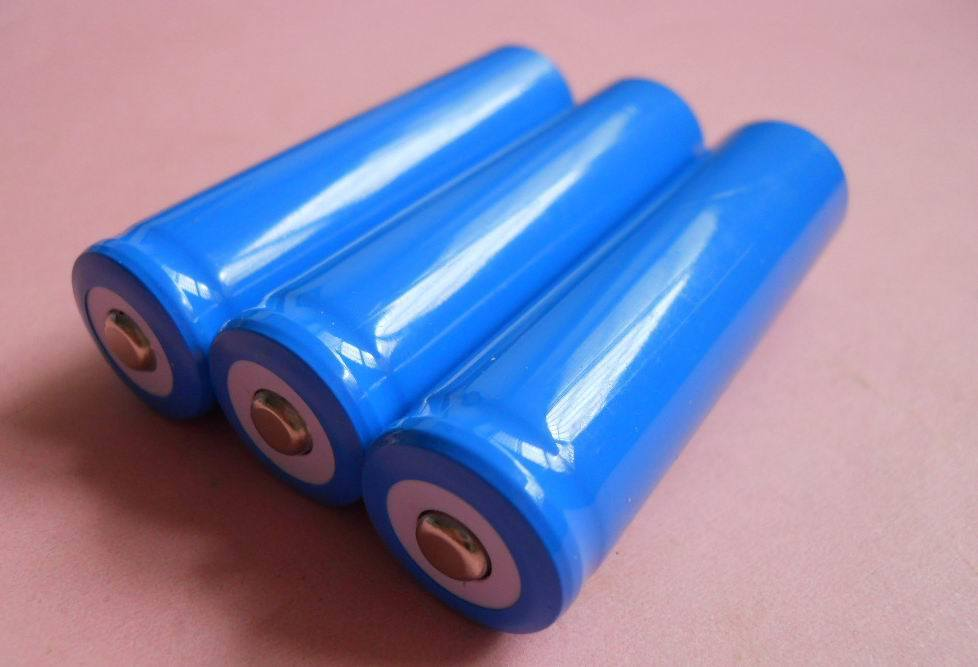
\includegraphics[width=0.8\textwidth]{figures/ogniwa.jpg}
	\caption{Ogniwa 16850}
	\label{fig:ogniwa}
\end{figure}



\subsection{Balanser}

Do zarządzania ogniwami użyty zostanie gotowy układ BMS przystosowany do współpracy z trzema ogniwami 16850. 
Zapewnia on podstawowe zabezpieczenia w tym:

\begin{itemize}
	\item zabezpieczenie przed nadmiernym rozładowaniem poniżej 3.0V,
	\item zabezpieczenie przed przeładowaniem powyżej 4.25V,
	\item zabezpieczenie przed przeciążeniem prądowym,
	\item zabezpieczenie przed zwarciem.
\end{itemize}

Napięcie generowane przez baterię ogniw powinno oscylować w zakresie 9.0V - 12.7V

\begin{figure}[H]
	\centering
	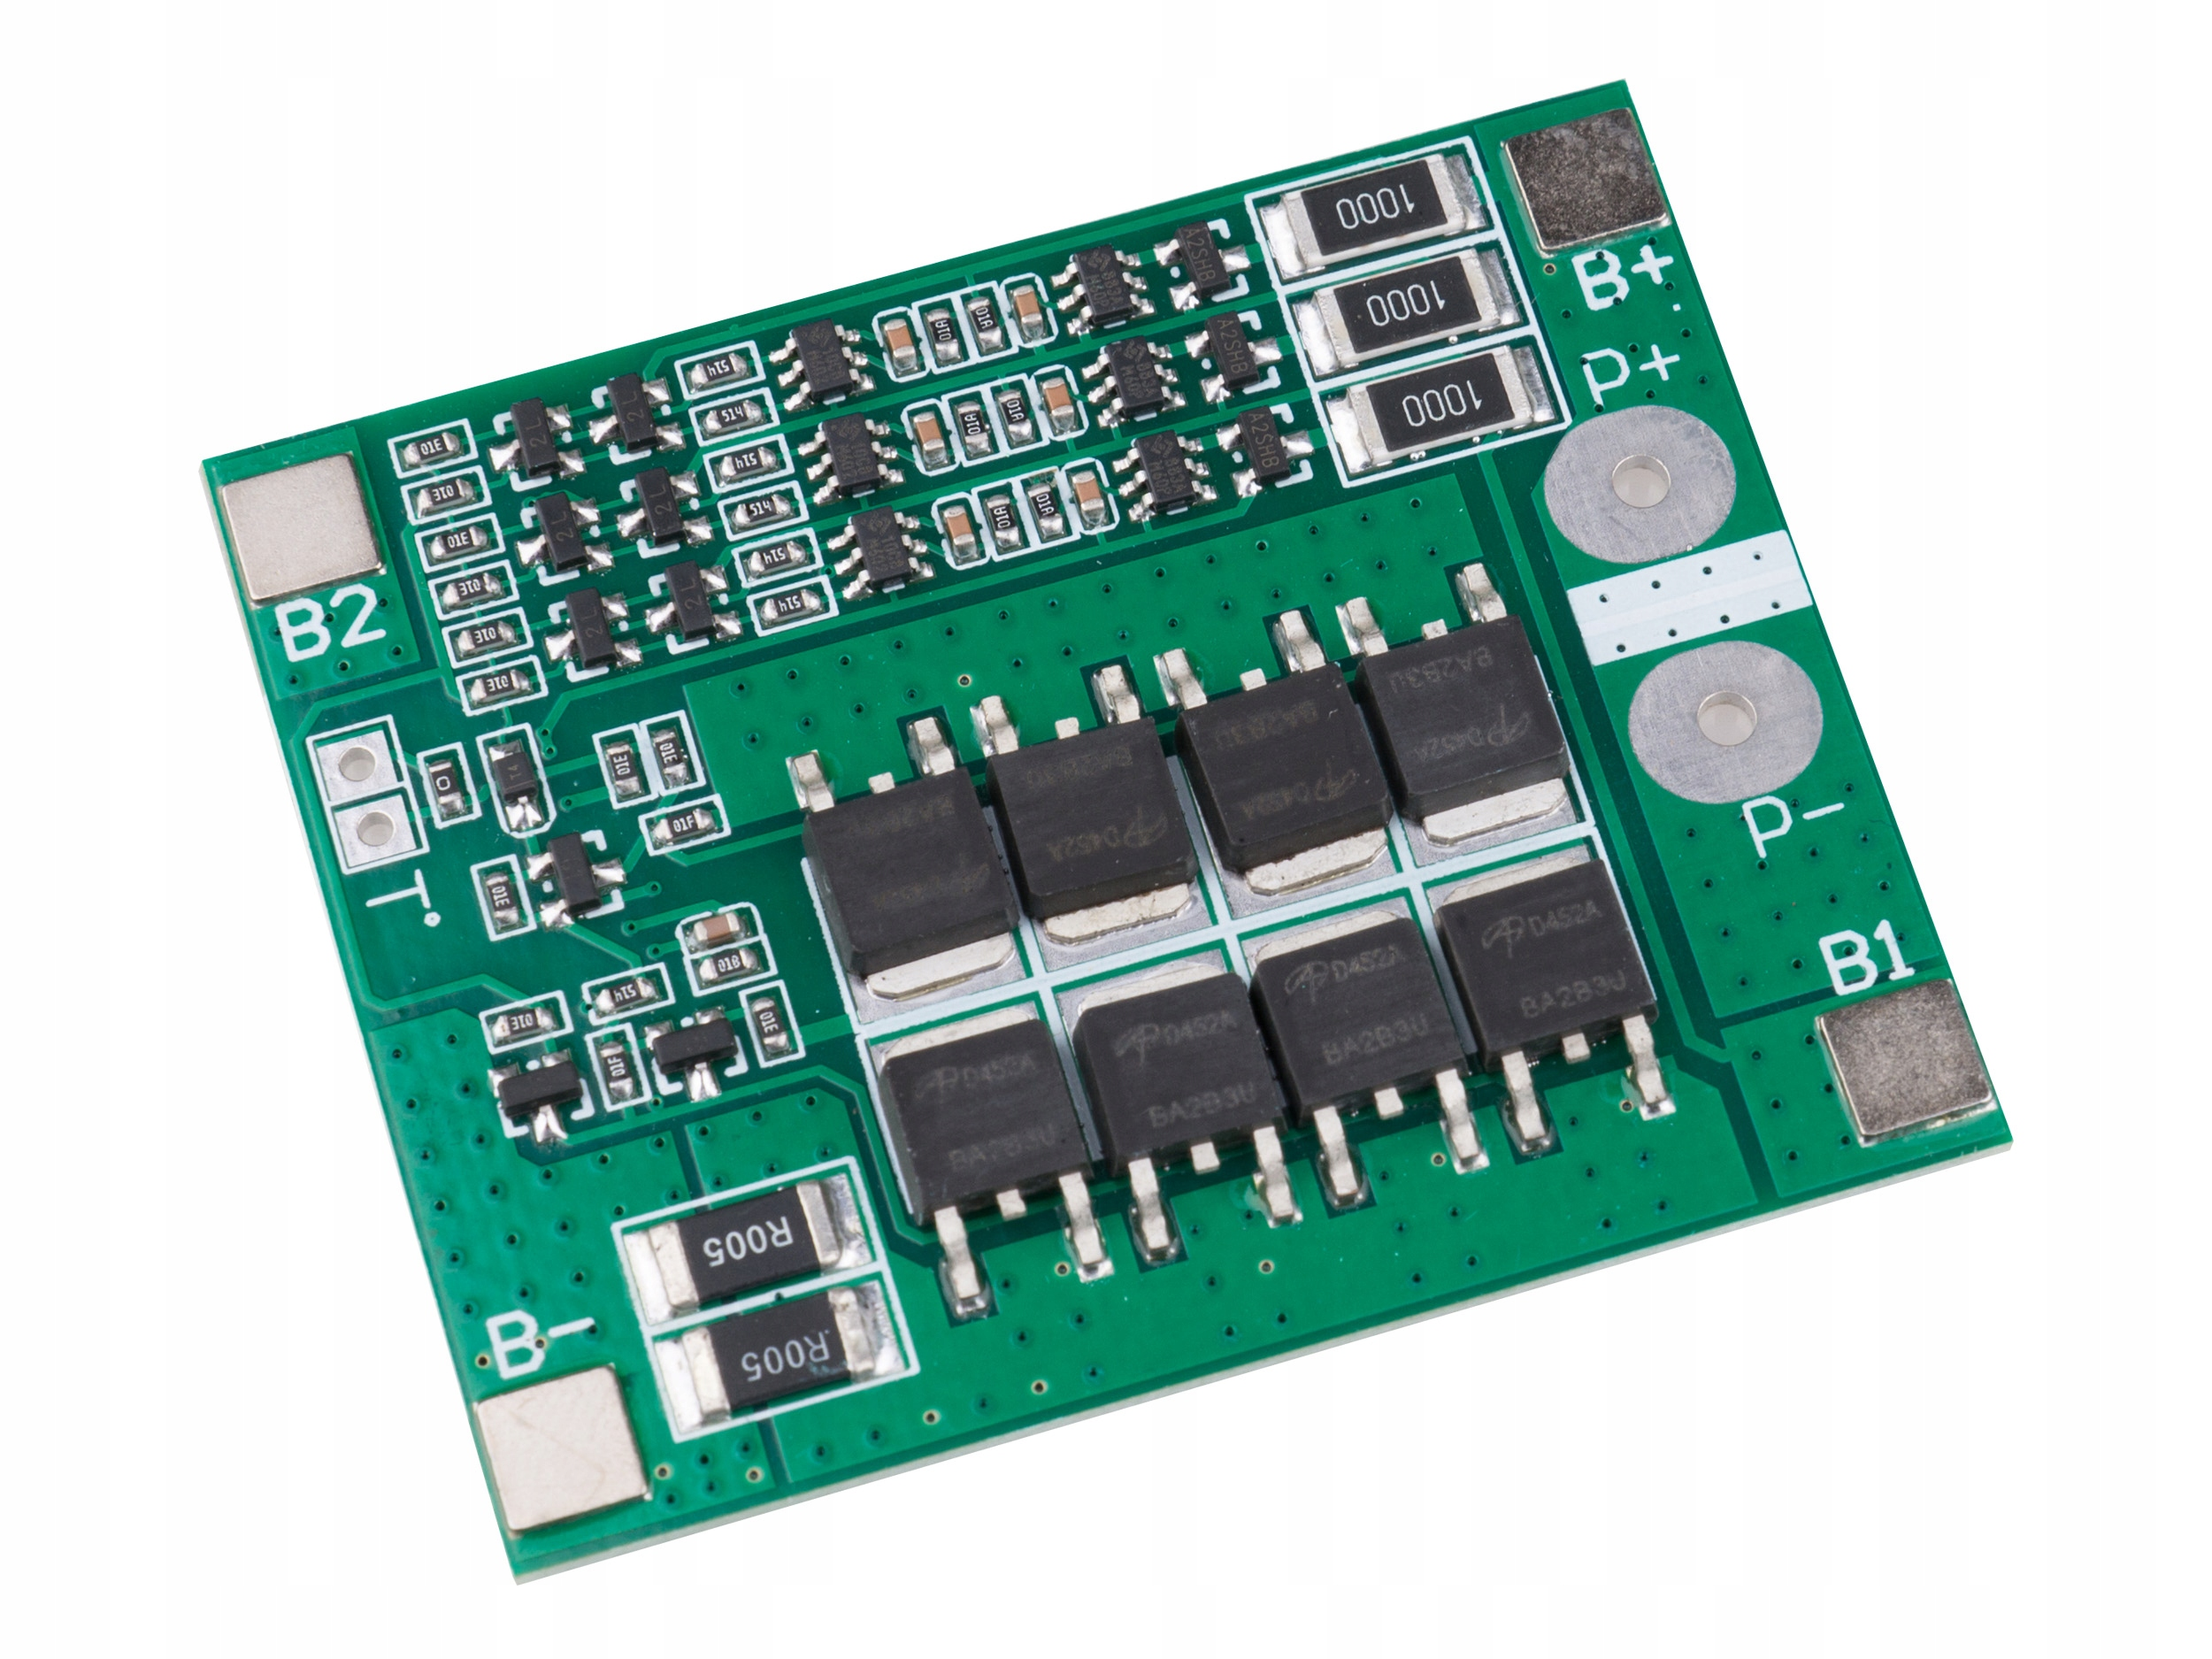
\includegraphics[width=0.6\textwidth]{figures/bms.jpg}
	\caption{Balanser baterii}
	\label{fig:bms}
\end{figure}


\section{Płytka drukowana}
Jednym z podstawowych elementów projektu jest stworzenie płytki drukowanej integrującej wszystkie wymagane elementy.

\subsection{Mikrokontroler}
Sercem układu zostanie układ ESP32-WROVER. 
Najważniejszym kryterium decydującym o wyborze tego konkretnego układu jest wbudowany modu WiFi i jego niska cena oscylująca w okolicach 2.50\$.
Jest to zdecydowanie najtańszy sposób na połączenia robota do Internetu.

\begin{figure}[H]
	\centering
	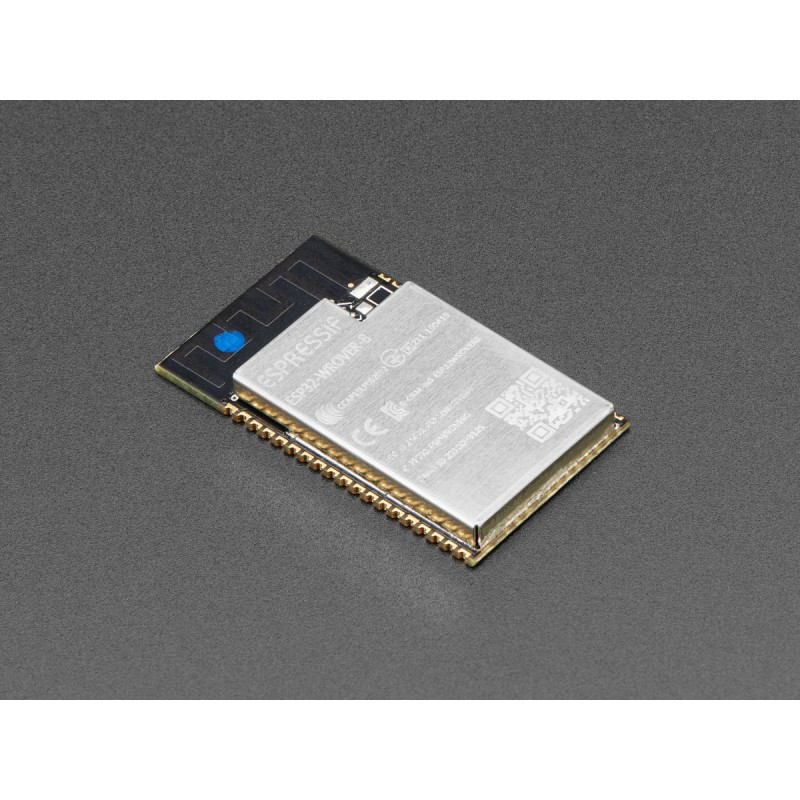
\includegraphics[width=0.65\textwidth]{figures/esp.jpg}
	\caption{Mikrokontroler ESP32}
	\label{fig:esp32}
\end{figure}

Najważniejsze cechy:
\begin{itemize}
	\item Wbudowany MCU o dwóch rdzeniach z taktowaniem do 240 MHz
	\item Protokoły Wi-Fi: 802.11 b/g/n/d/e/i/k/r
	\item Protokoły BT: Bluetooth v4.2 BR/EDR oraz Bluetooth BLE
	\item Napięcie zasilania: 2.2 V - 3.6 V
	\item Średni pobór prądu: 80 mA
\end{itemize}

\subsection{Sterowniki silników}
Układ będzie wspierał sterowanie dwoma silnikami prądu stałego. 
Każdy z nich będzie mógłbyć wyposarzony w osobny enkoder liczący obroty silnika.
Do tego celu posłuży układa L298N w obudowie Multiwatt 15 pin.

\begin{figure}[H]
	\centering
	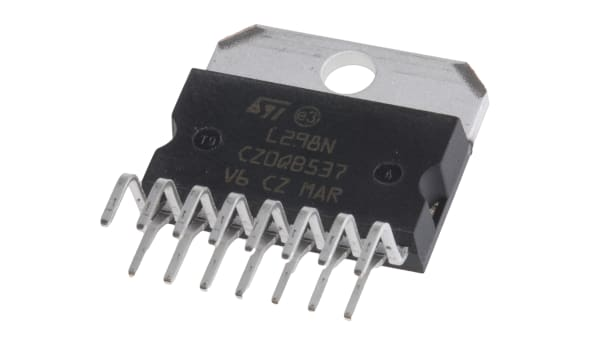
\includegraphics[width=0.65\textwidth]{figures/l298.jpg}
	\caption{Układ scalony L298N}
	\label{fig:l298n}
\end{figure}

\subsection{Akcelereometr}
Robot będzie wyposarzony w akcelerometr i żyroskop, aby móc mierzyć przyspieszenia oraz prędkości kątowe.
Będzie to możliwe dzięki użyciu układu MPU-6050.

\begin{figure}[H]
	\centering
	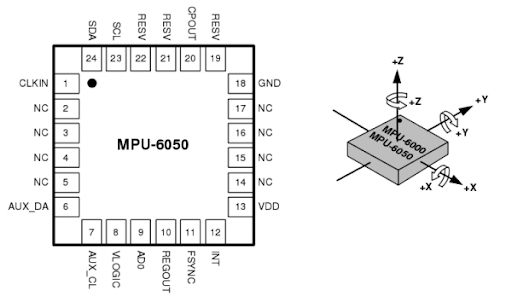
\includegraphics[width=0.7\textwidth]{figures/mpu6050.png}
	\caption{Układ scalony MPU6050}
	\label{fig:mpu6050}
\end{figure}

\subsection{Inne}
Aby móc komfortowo użytkować i prototypować robota niezbędne będą dodatkowe elementy takie jak:
\begin{itemize}
	\item wyprowadzenie JATG,
	\item wyprowadzenie interfejsu I2C,
	\item wyprowadzenie kamery ArduCam OV2640,
	\item wyprowadzenie UART,
	\item wejście zasilania,
	\item złącze czujnika ultradzwiękowego,
	\item dwa wejścia enkoderów,
	\item dwa wyjścia na silniki.
\end{itemize}

\section{Mechanika}
\subsection{Podwozie}
Aby zredukować koszty i lepiej zintegrować wszystkie elementy ze sobą,
postanowiłem samemu zaprojektować podwozie i wydrukować je przy użyciu drukarki 3D.
Materiał który do tego użyję to ABS.
% Na początku planowania projektu miałem zamiar zaprojektować własne podwozie, 
% ale koszty silników z enkoderami były bardzo duże. Bardziej opłacalne okazały się gotowe zestawy,
% więc zdecydowałem że jako podwozie zostanie użyty zestaw "4WD Smart Robot Car Chassis Kits".
% Jest to najbardziej opłacalne rozwiązanie.

\subsection{Silniki}
Silniki których użyję są produkcji DFRobot. Mają one doczepione enkodery, 
które pozwolą mi bardzo dokładnie kontorlować prędkości silników.
\begin{figure}[H]
	\centering
	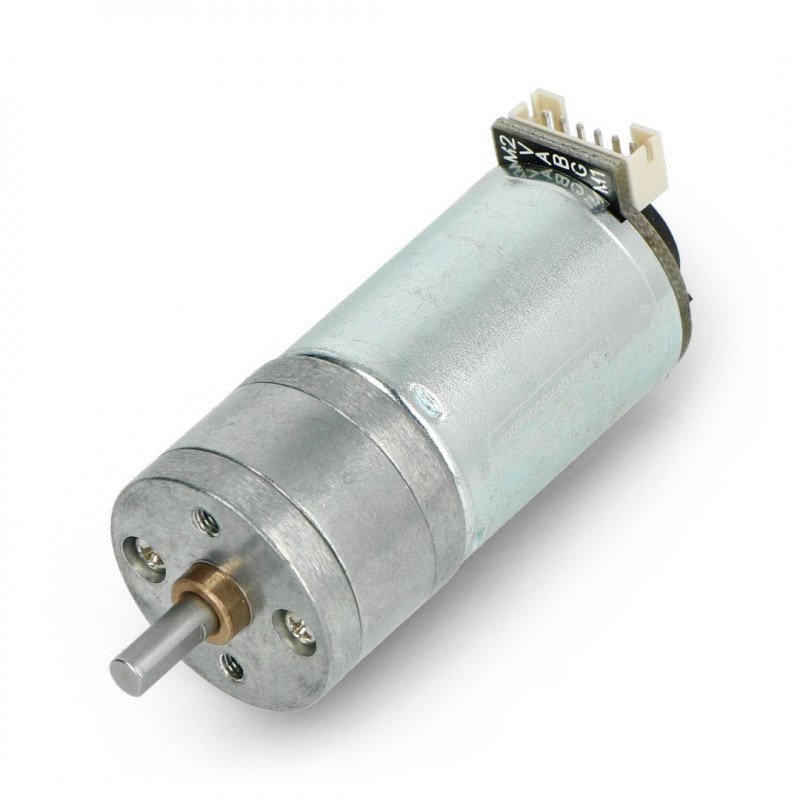
\includegraphics[width=0.7\textwidth]{figures/silnik.png}
	\caption{Silnik z enkoderem}
	\label{fig:silnk}
\end{figure}

Ich skrócona specyfikacja:
\begin{itemize}
	\item Napięcie zasilania: 6 V
	\item Napięcie enkodera: od 3,3 V do 5 V
	\item Współczynnik redukcji: 1:20
	\item Prędkość bez obciążenia: 300 RPM - 0,1 A
\end{itemize}

\section{Harmonogram}
\begin{enumerate}
	\item Sporządzenie listy i zdobycie wymaganych elementów. (17.03)
	\item Zaprojektowanie i wykonanie podwozia. (24.03)
	\item Zaprojektowanie i wykonanie pakietu baterii. (31.03)
	\item Zaprojektowanie płytki drukowanej. (7.04)
	\item Napisanie i przetestowanie bazowej wersji programu na MCU. (14.04)
	\item Zbudowanie komunikacji z kontrolerem. (21.04)
	\item Dodanie obsługi enkoderów. (28.04)
	\item Dodanie obsługi żyroskopu. (5.05)
	\item Testowanie i dopieszczanie. (12.05)
\end{enumerate}


\section{Podwozie}
Podwozie zostało zaprojektowane w programie Fusion360. 
Pierwsza wersja cierpiała na problemy związane z małą sztywnością 
konstrukcji, co znacząco wpływało na jakość sterowania. 
Z tego też powodu została zaprojektowana druga, znacznie wytrzymalsza
wersja podwozia.

\begin{figure}[H]
	\centering
	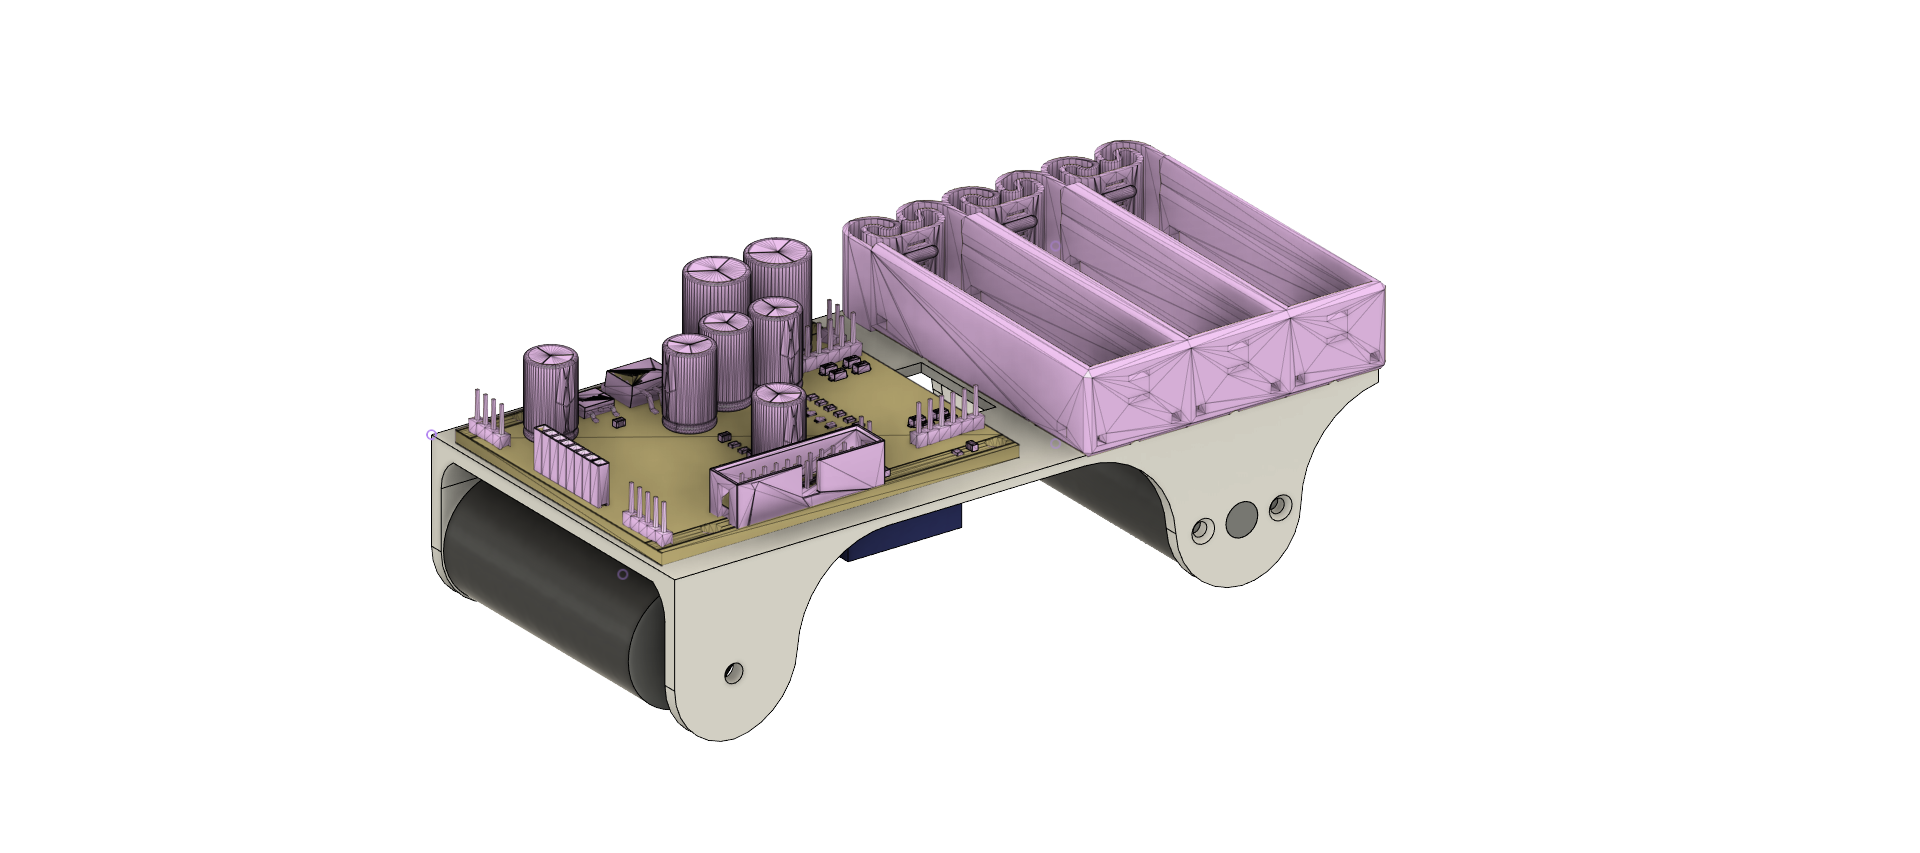
\includegraphics[width=1\textwidth]{figures/chassisV1.png}
	\caption{Pierwsza wersja podwozia}
	\label{fig:chassisv1}
\end{figure}

\begin{figure}[H]
	\centering
	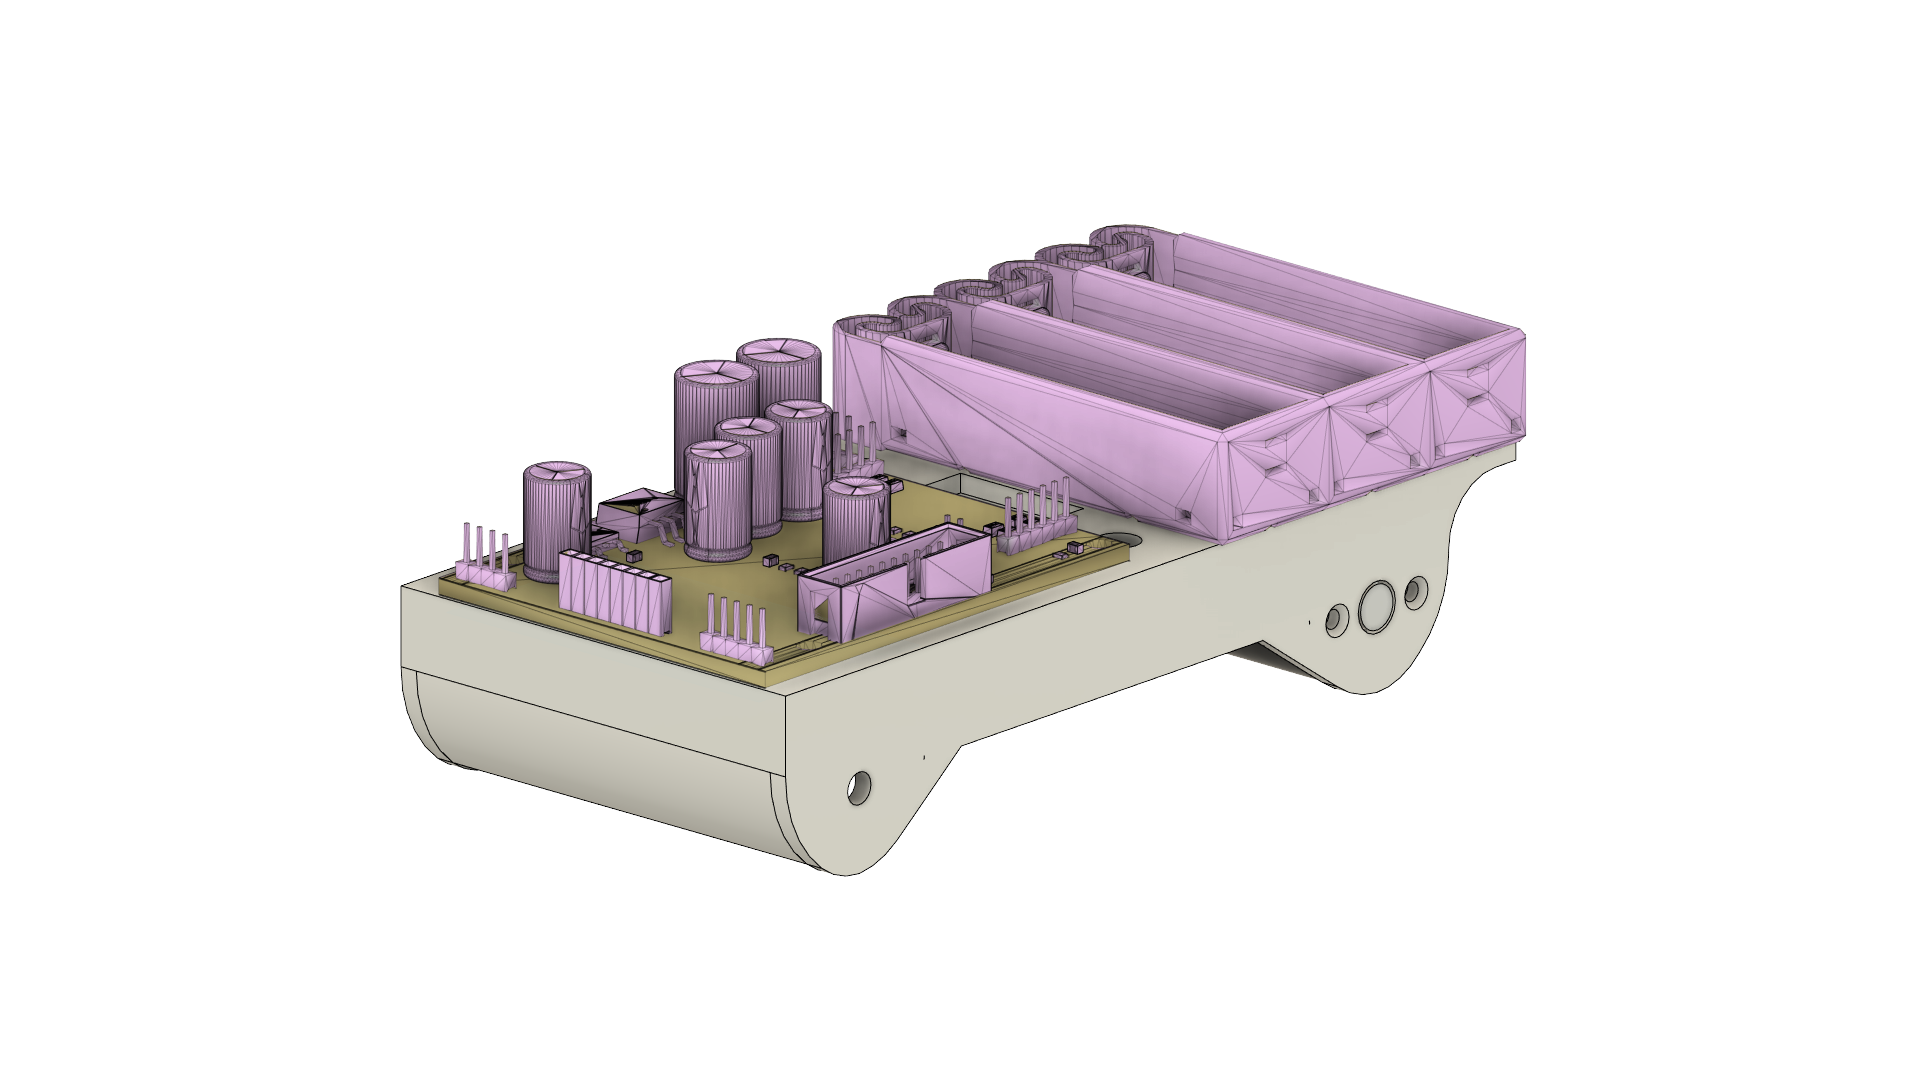
\includegraphics[width=1\textwidth]{figures/chassisV2.png}
	\caption{Druga wersja podwozia}
	\label{fig:chassisv2}
\end{figure}


\section{Płytka drukowana}
W celu zwiększenia jakości i poprawy niezawodności projektu, 
została zaprojektowana płytka drukowana, która ma za zadanie
integrować wszystkie niezbędne peryferia i minimalzować zajmowane miejsce. 

\begin{figure}[H]
	\centering
	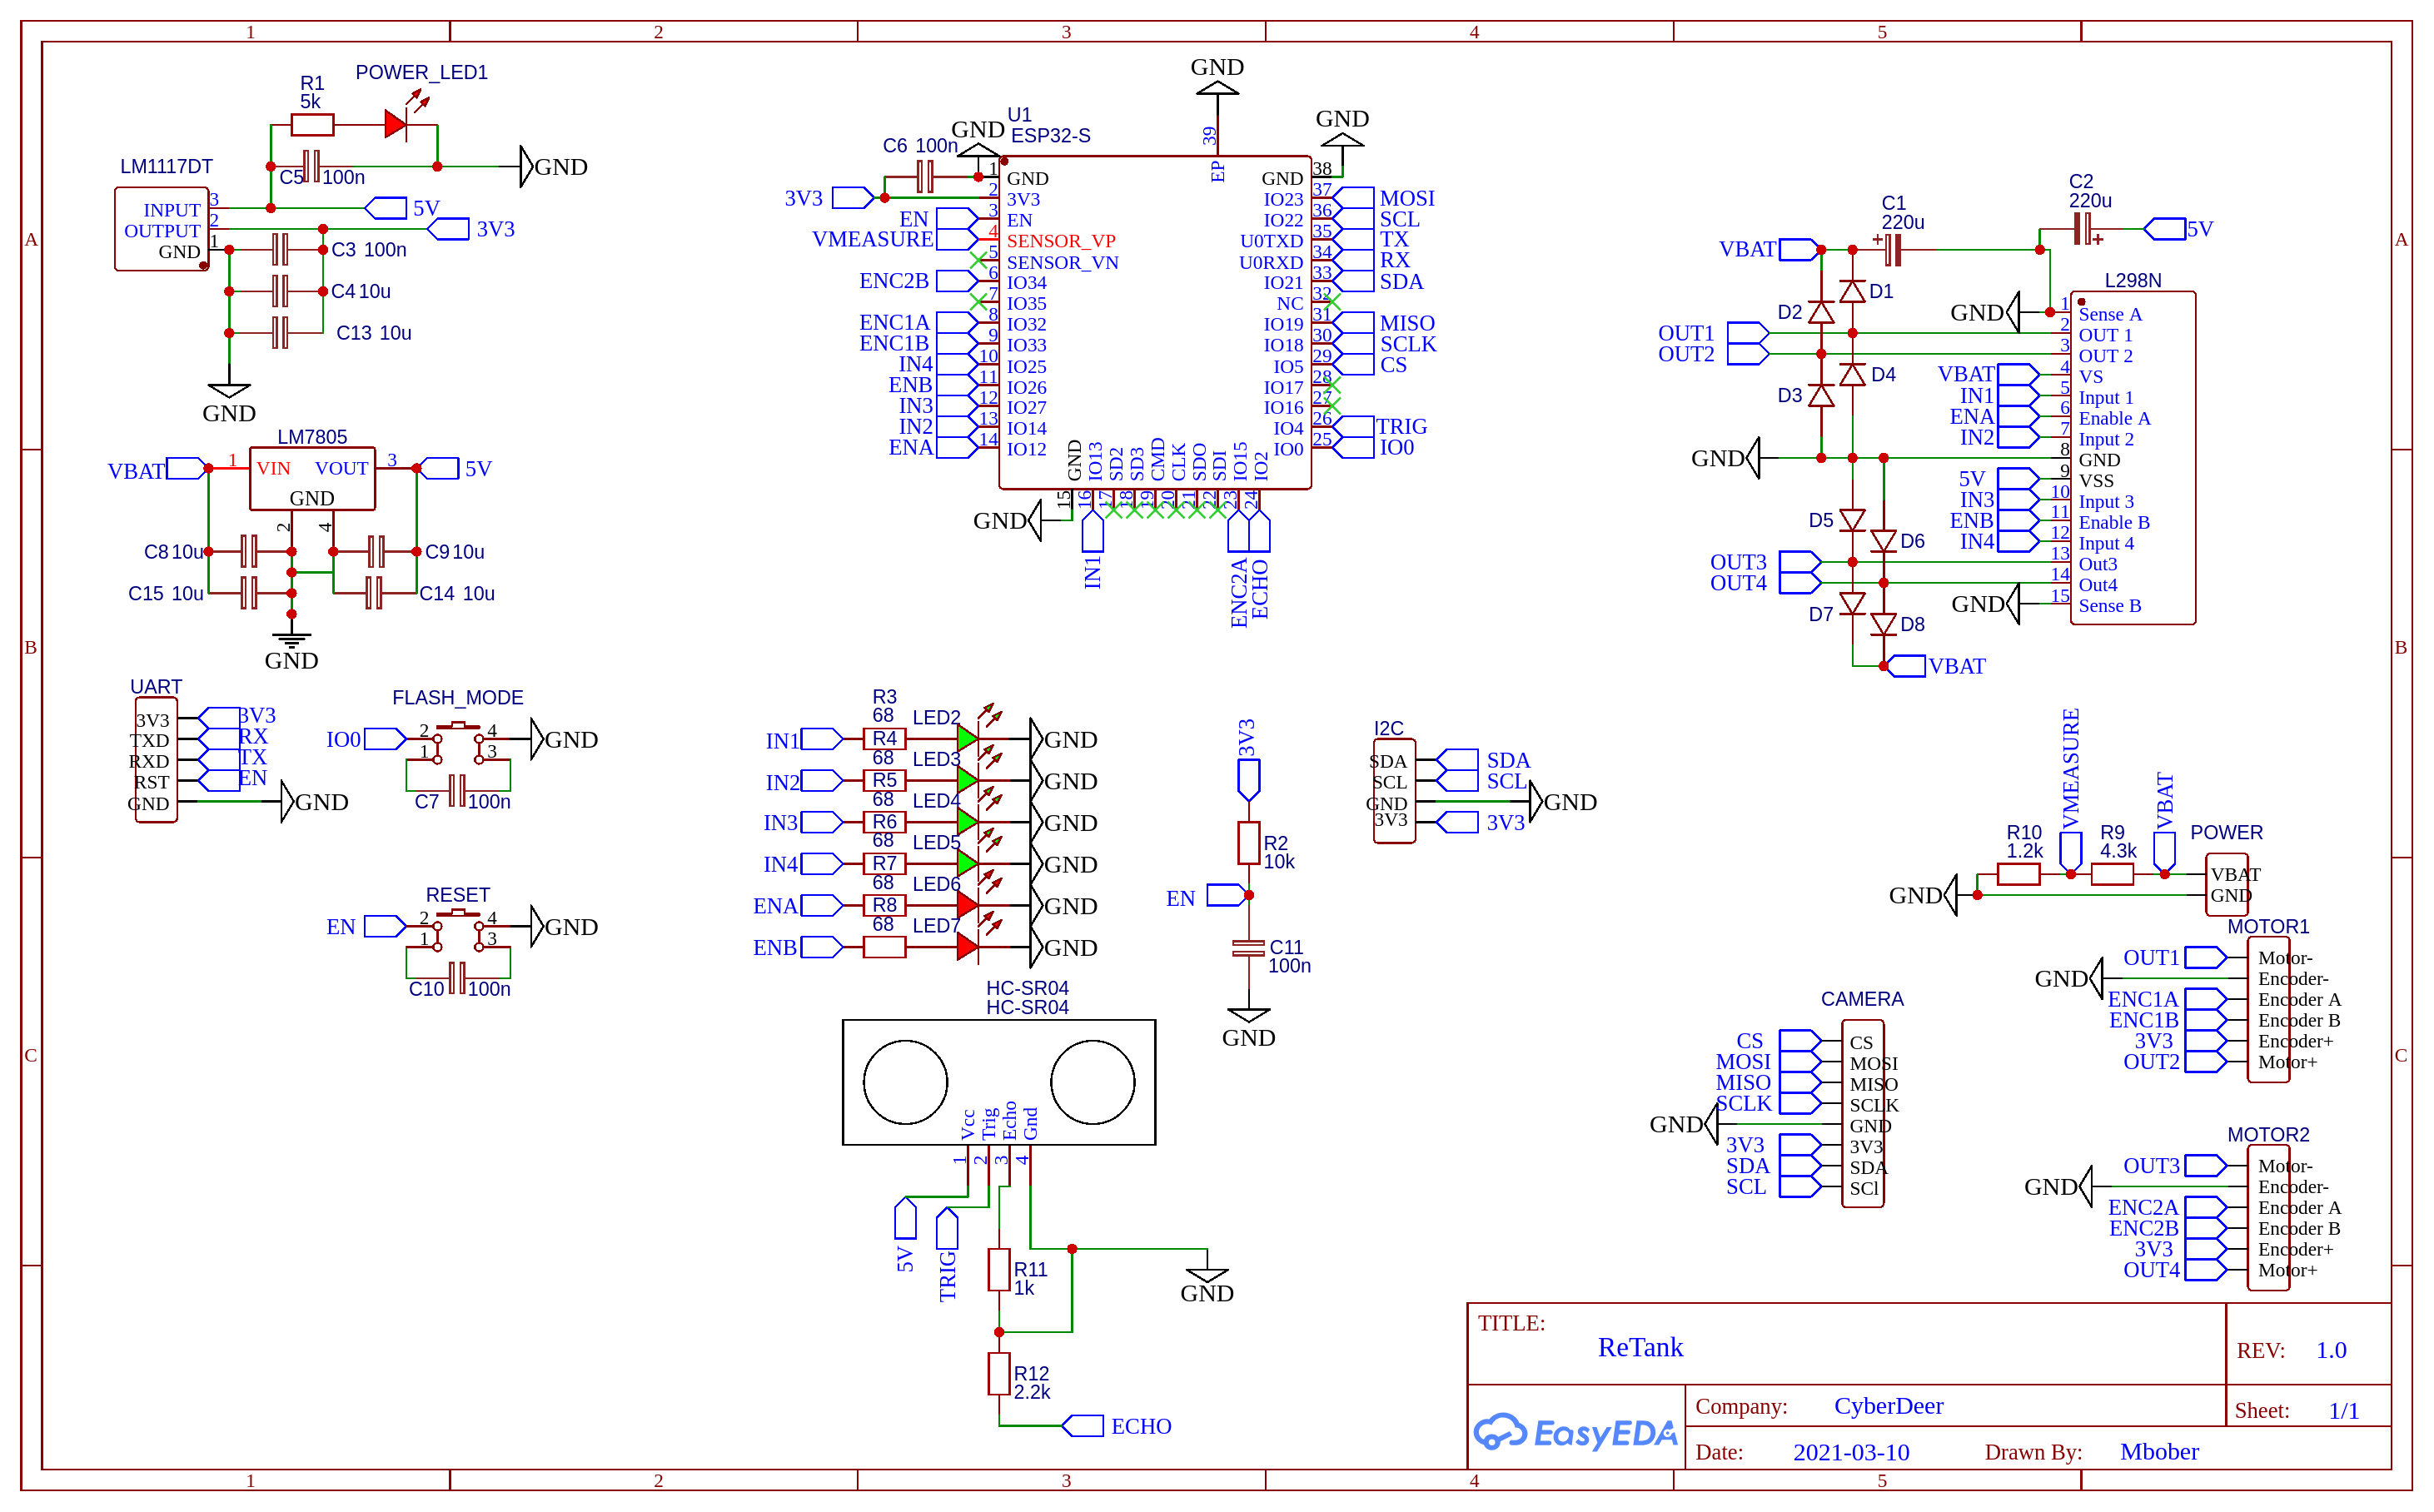
\includegraphics[width=1\textwidth]{figures/schematic.png}
	\caption{Schemat połączeń}
	\label{fig:schematic}
\end{figure}

2021-04-16 zostało złożone zamówienie na 5 sztuk płytek.
Zamówienie jest jeszcze w trakcie transportu. Ostateczną wersję 
można zobaczyć poniżej. Z powodu ograniczonej przestrzeni i
niewystarczającej liczby pinów mikrokontrolera, zrezygnowałem z
portu JTAG.

\begin{figure}[H]
	\centering
	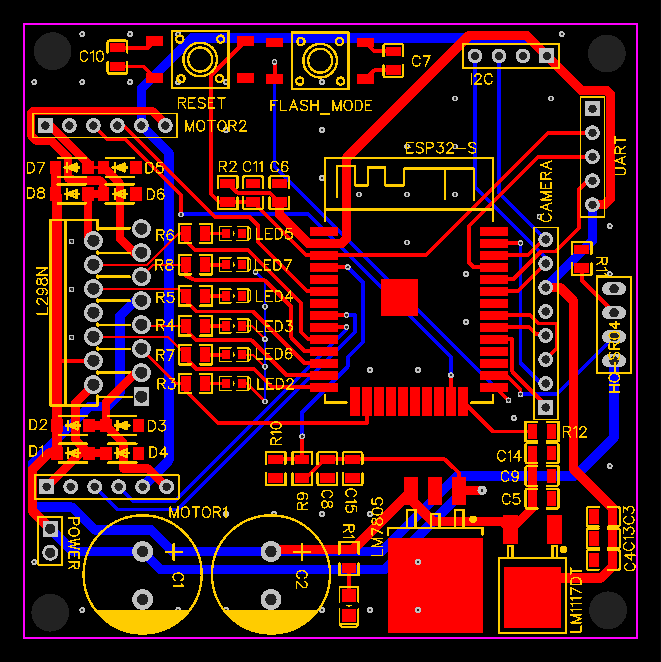
\includegraphics[width=0.5\textwidth]{figures/pcb.png}
	\caption{PCB}
	\label{fig:pcb}
\end{figure}


\section{Program}
Program na mikrokontroler został napisany z użyciem warstwy abstrakcji
ESP-IDF, udostępnionej przez producenta układu. Dla zwiększenia 
możliwości sprzętu, zdecydowałem się na użycie systemu czasu rzeczywistego
FreeRTOS. Dzięki temu kod został podzielony na oddzielne moduły, 
a każdy z nich pracuje na swoim odrębnym wątku. Pozwoliło to również
ustawiać wyższy piorytet funkcjom, które mają krytyczny wpływ na dzianie robota.
Komunikacja międzyprocesowa została zrealizowana poprzez kolejki piorytetowe,
co znacząco usprawnia cały proces.

Całość kodu dostępna jest w moim repozytorium na
\href{https://github.com/mbober1/ReTank}{GitHub}.

\section{Komunikacja z robotem}

Połączenie z robotem odbywa się poprzez sieć WiFi. W pierwszej kolejności 
nawiązywane jest połączenie przy użyciu protokołu TCP. Jeśli się ono powiedzie
to uruchamiana jest dodatkowa transmicja z wykorzystaniem UDP. 
Dzięki takiej koncepcji mamy dwa niezależne kanały komunikacji. Pierwszy służy
do przesyłania danych które mają niski piorytet czasowy, potrzebują potwierdzenia
odebrania i ewentualnej retransmisji danych. Druga droga komunikacji powstała, 
aby przesyłać ciągły strumień nowych danych. Zależy nam na jaknajniższym opóźnieniu,
a ewentualny błąd trasmisji nie jest krytyczny, bo inforamcje te szybko się 
przedawniają i są zastępowane przez nowe, świeższe. \newline

Każda ramka zaczyna się od wybranej dużej litery alfabetu, określającej rodzaj 
przesyłanych danych. Dla protokołu TCP są to:

	\begin{itemize}
	  \item P - ping,
	  \item D - dystans przeszkody,
	  \item B - bateria,
	  \item S - realna predkość.
	\end{itemize}
	
Natomiast dla protokołu UDP wyróżniamy:
  \begin{itemize}
	\item E - moc silników,
	\item A - akcelometr,
	\item G - żyroskop.
  \end{itemize}

Wszystkie paczki danych zakończone są średnikiem, przed którym znajduje się
ośmiobitowy cykliczny kod nadmiarowy. Niestety ze względu na róźnorodność 
transmitownych informacji, w tym miejscu kończą się cechy wspólne poszczególnych 
ramek.

\subsection{Ping}
Jest to najprostrza z obecych tu ramek. Nie przenosi żadnych informacji.
Oznacza jedynie koniecność odesłania do nadawcy identyczniej wiadomości,
aby można było wyznaczyć chwilę czasowe, niezbędne do obliczenia opóźnienia
transmisji.

Forma ramki to: $P\#;$

Gdzie \# oznacza CRC.



\subsection{Dystans przeszkody}
Przesyła informacje z robota o odległości odczytanej z czujnika ultradzwiękowego.

Forma ramki to: $D<uint8\_t>\#$;
\newline

Gdzie \# oznacza CRC. Przed nim znajduje się wartość odległości wyrażonej 
w centymetrach, w zakresie 0-100cm.



\subsection{Bateria}
Przesyła informacje z robota o poziomie baterii.

Forma ramki to: $B<uint8\_t>\#$;
\newline

Gdzie \# oznacza CRC. Przed nim znajduje się poziom baterii wyrażonej 
w procentach, w zakresie 0-100\%.



\subsection{Prędkość}
Przesyła informacje z robota o prędkości na kołach.

Forma ramki to: $S<uint8\_t> <uint8\_t>\#$;
\newline

Gdzie \# oznacza CRC. Przed nim znajdujdują się dwie wartości oddzielone spacją
odnoszące się do prędkości poszczególnych kół wyrażonej w metrach na sekunde.



\subsection{Moc silników}
Przesyła informacje z aplikacji do robota o zadanej mocy silników.

Forma ramki to: $E<uint8\_t> <uint8\_t>\#$;
\newline

Gdzie \# oznacza CRC. Przed nim znajdujdują się dwie wartości oddzielone spacją
odnoszące się do zadanej mocy poszczególnych kół wyrażonej w procentach.
Zakresy tych wartości musza mieścić się od 0 do 100\%



\subsection{Akcelometr}
Przesyła informacje z robota o aktualnych wskazaniach akcelometru.

Forma ramki to: $A<uint8\_t> <uint8\_t> <uint8\_t>\#$;
\newline

Gdzie \# oznacza CRC. Przed nim znajdujdują się trzy wartości oddzielone spacją
odnoszące się do aktualnych wskazań akcelometru.


\subsection{Żyroskop}
Przesyła informacje z robota o aktualnych wskazaniach żyroskopu.

Forma ramki to: $G<uint8\_t> <uint8\_t> <uint8\_t>\#$;
\newline

Gdzie \# oznacza CRC. Przed nim znajdujdują się trzy wartości oddzielone spacją
odnoszące się do aktualnych wskazań żyroskopu.


\section{Aplikacja do komunikacji}
Rezultaty komunikacji z komputerem i działania całego projektu możemy z
łatwością podziwiać z pomocą mojej specialnie przygotowanej aplikacji w QT
dostępnej w moim repozytorium na
\href{https://github.com/mbober1/RoboVision}{GitHub}.

\begin{figure}[H]
	\centering
	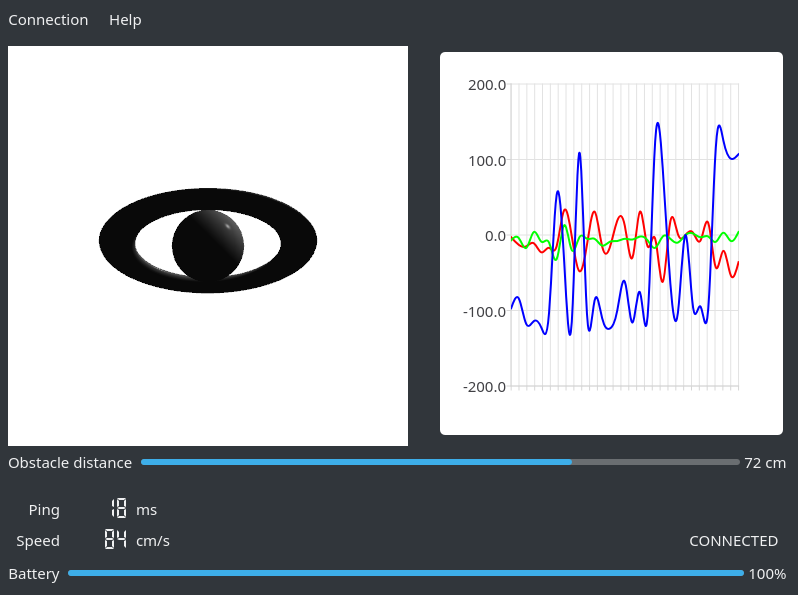
\includegraphics[width=1\textwidth]{figures/app.png}
	\caption{Aplikacja RoboVision}
	\label{fig:app}
\end{figure}


\begin{figure}[H]
	\centering
	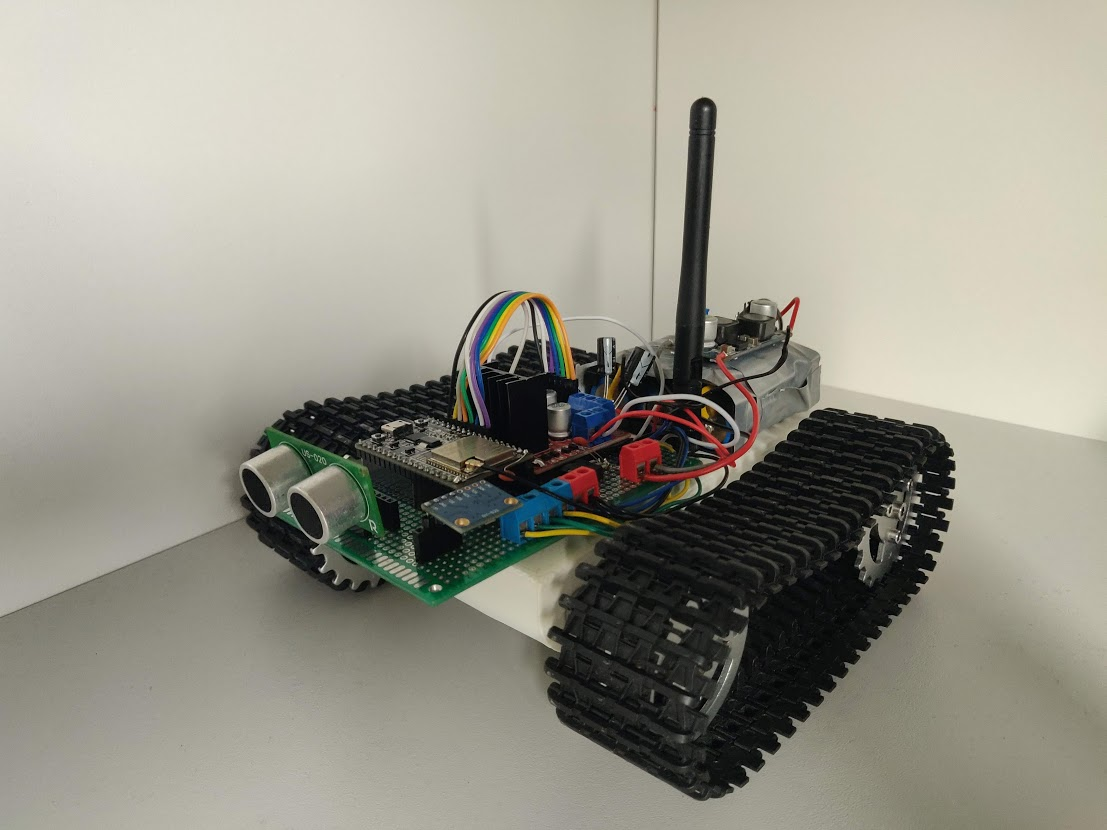
\includegraphics[width=1\textwidth]{figures/robotv1.jpg}
	\caption{Prototyp robota}
	\label{fig:robot}
\end{figure}

\section{Rezultat}
Projekt robota został zakończony sukcesem. Wszystkie problemy z jakimi borykały
się prototypy zostały wyeliminowane. Można więc uznać projekt za zamknięty.  

\begin{figure}[H]
	\centering
	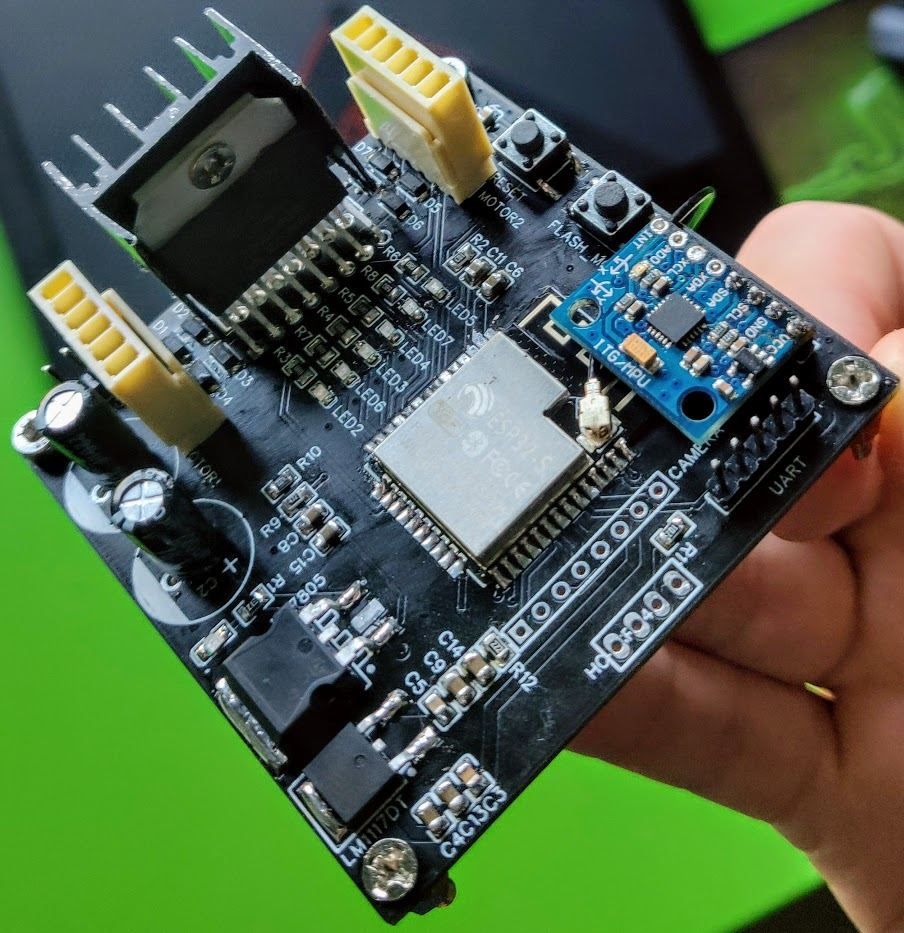
\includegraphics[width=0.7\textwidth]{figures/final/pcb.jpg}
	\caption{Ostateczna wersja płytki drukowanej}
	\label{fig:pcb_final}
\end{figure}

\begin{figure}[H]
	\centering
	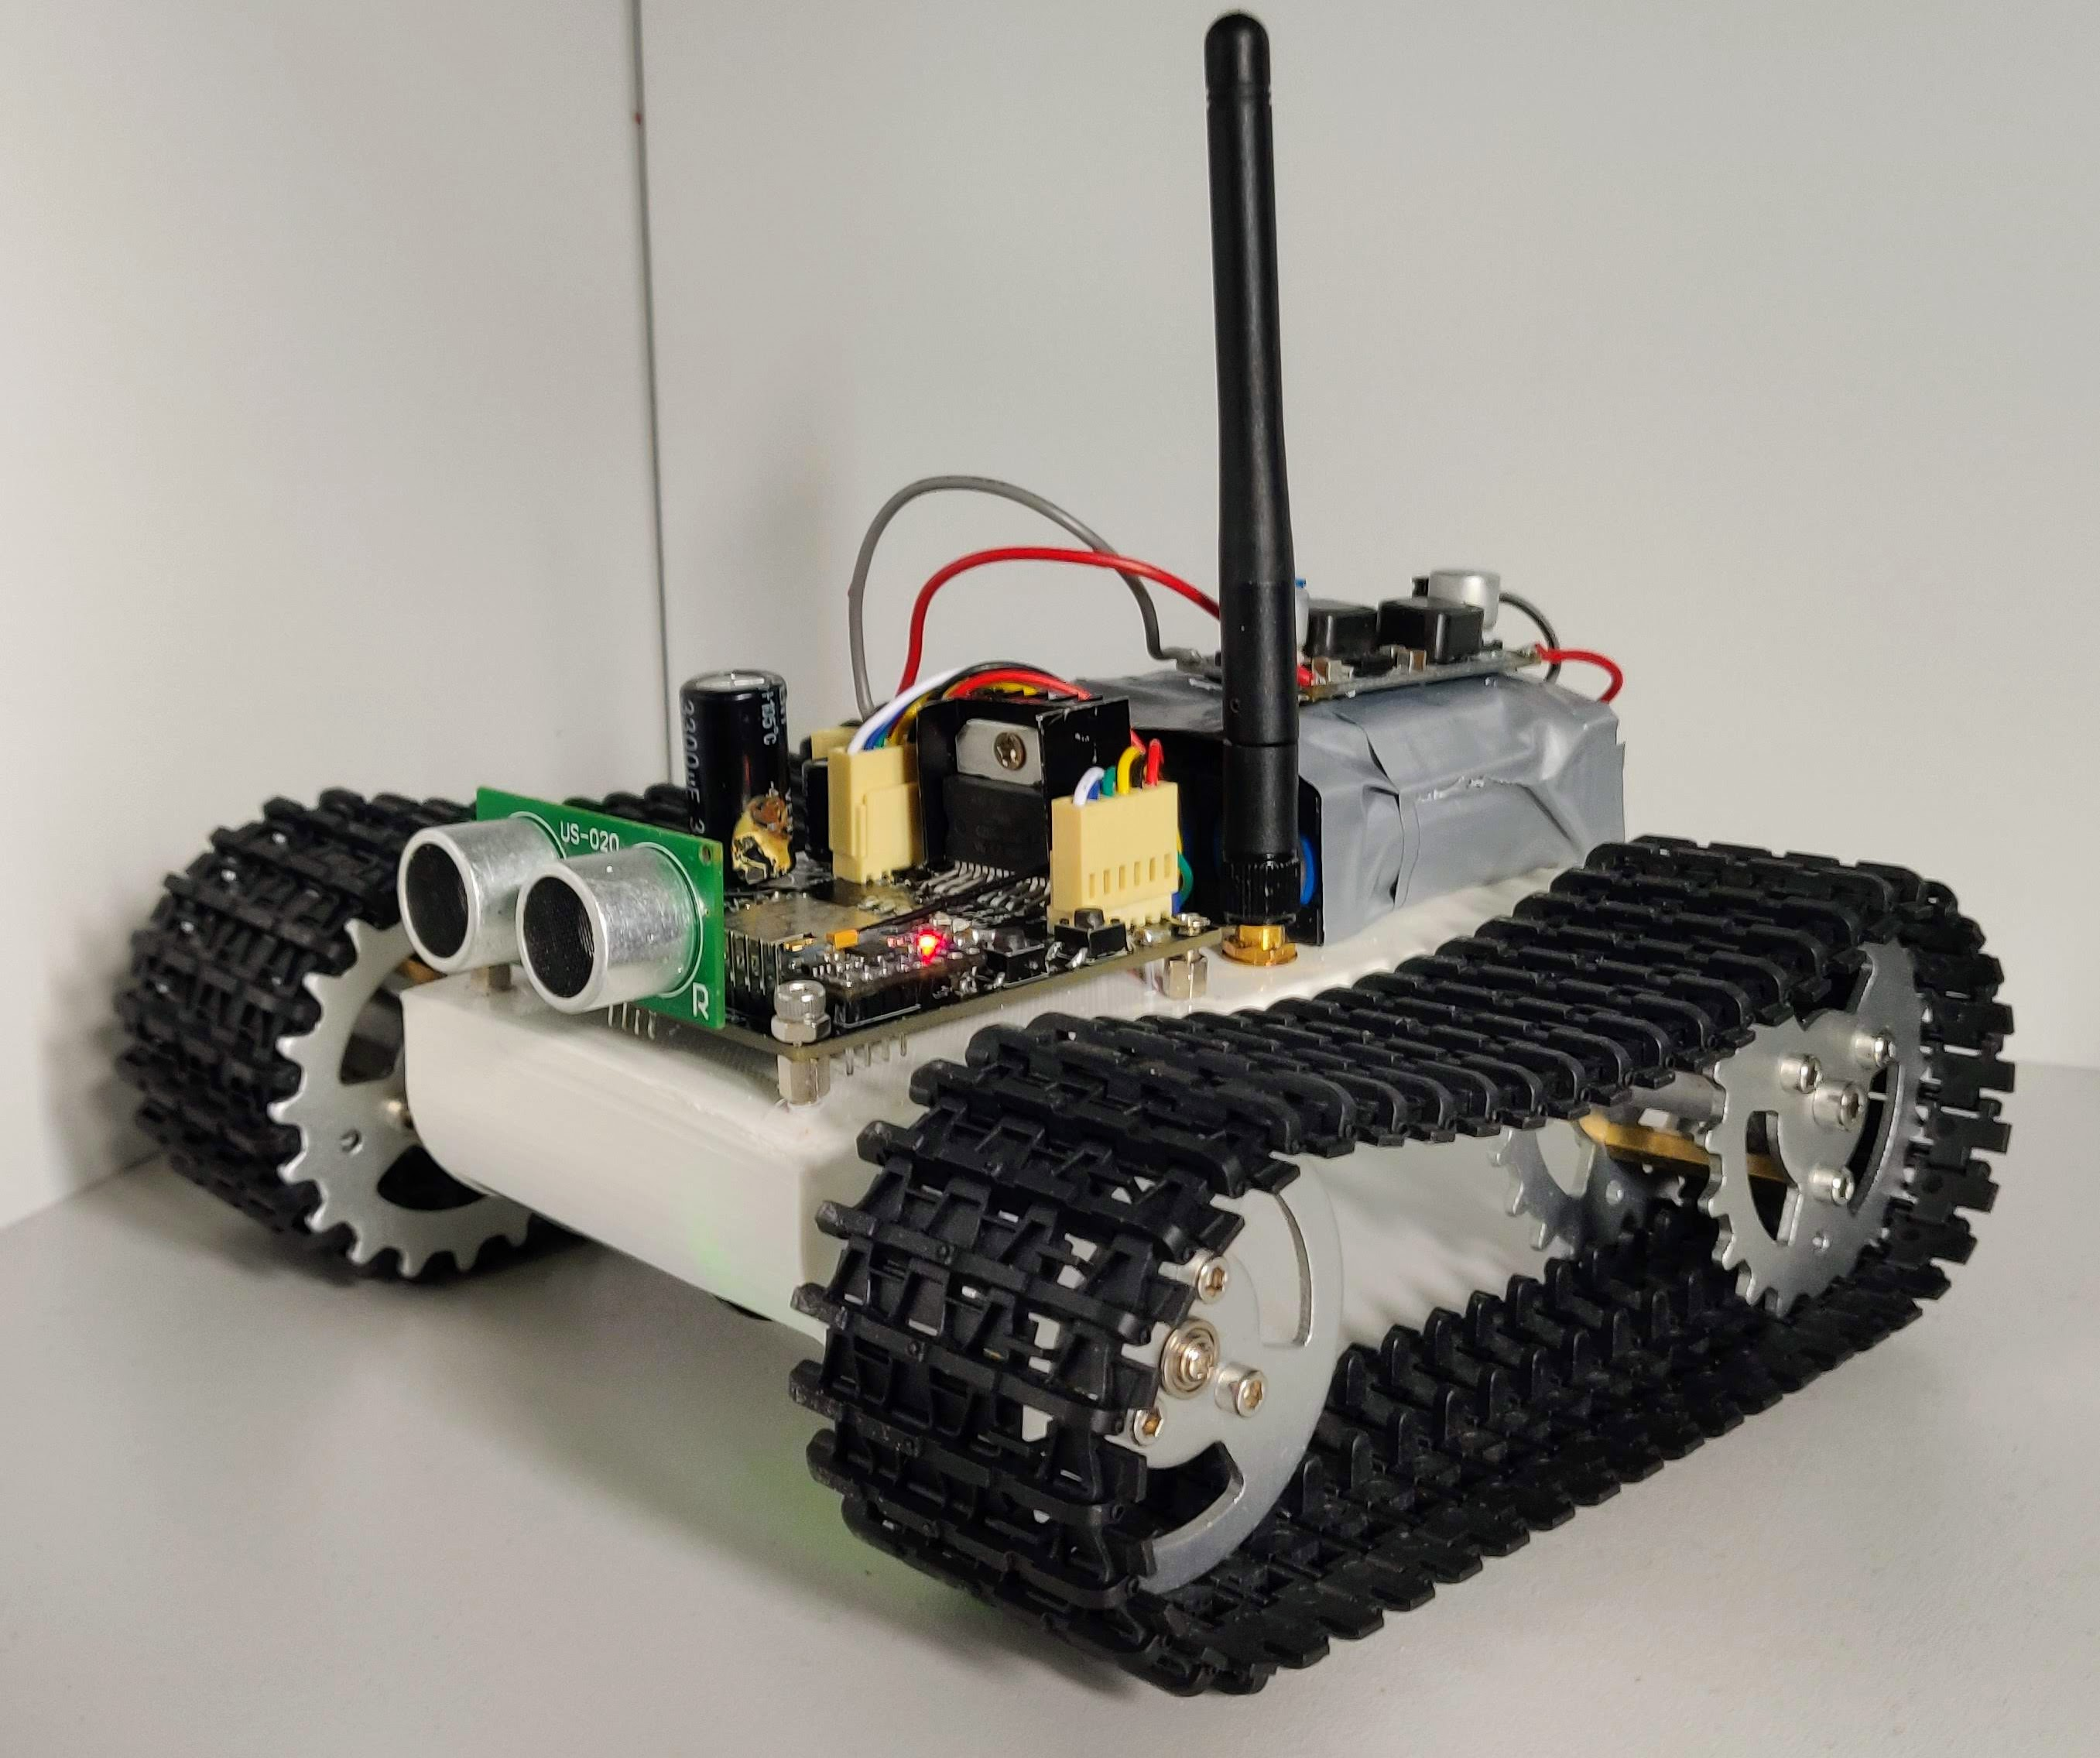
\includegraphics[width=0.7\textwidth]{figures/final/robot1.jpg}
	\caption{Ostateczna wersja robota}
	\label{fig:robot_final1}
\end{figure}

\begin{figure}[H]
	\centering
	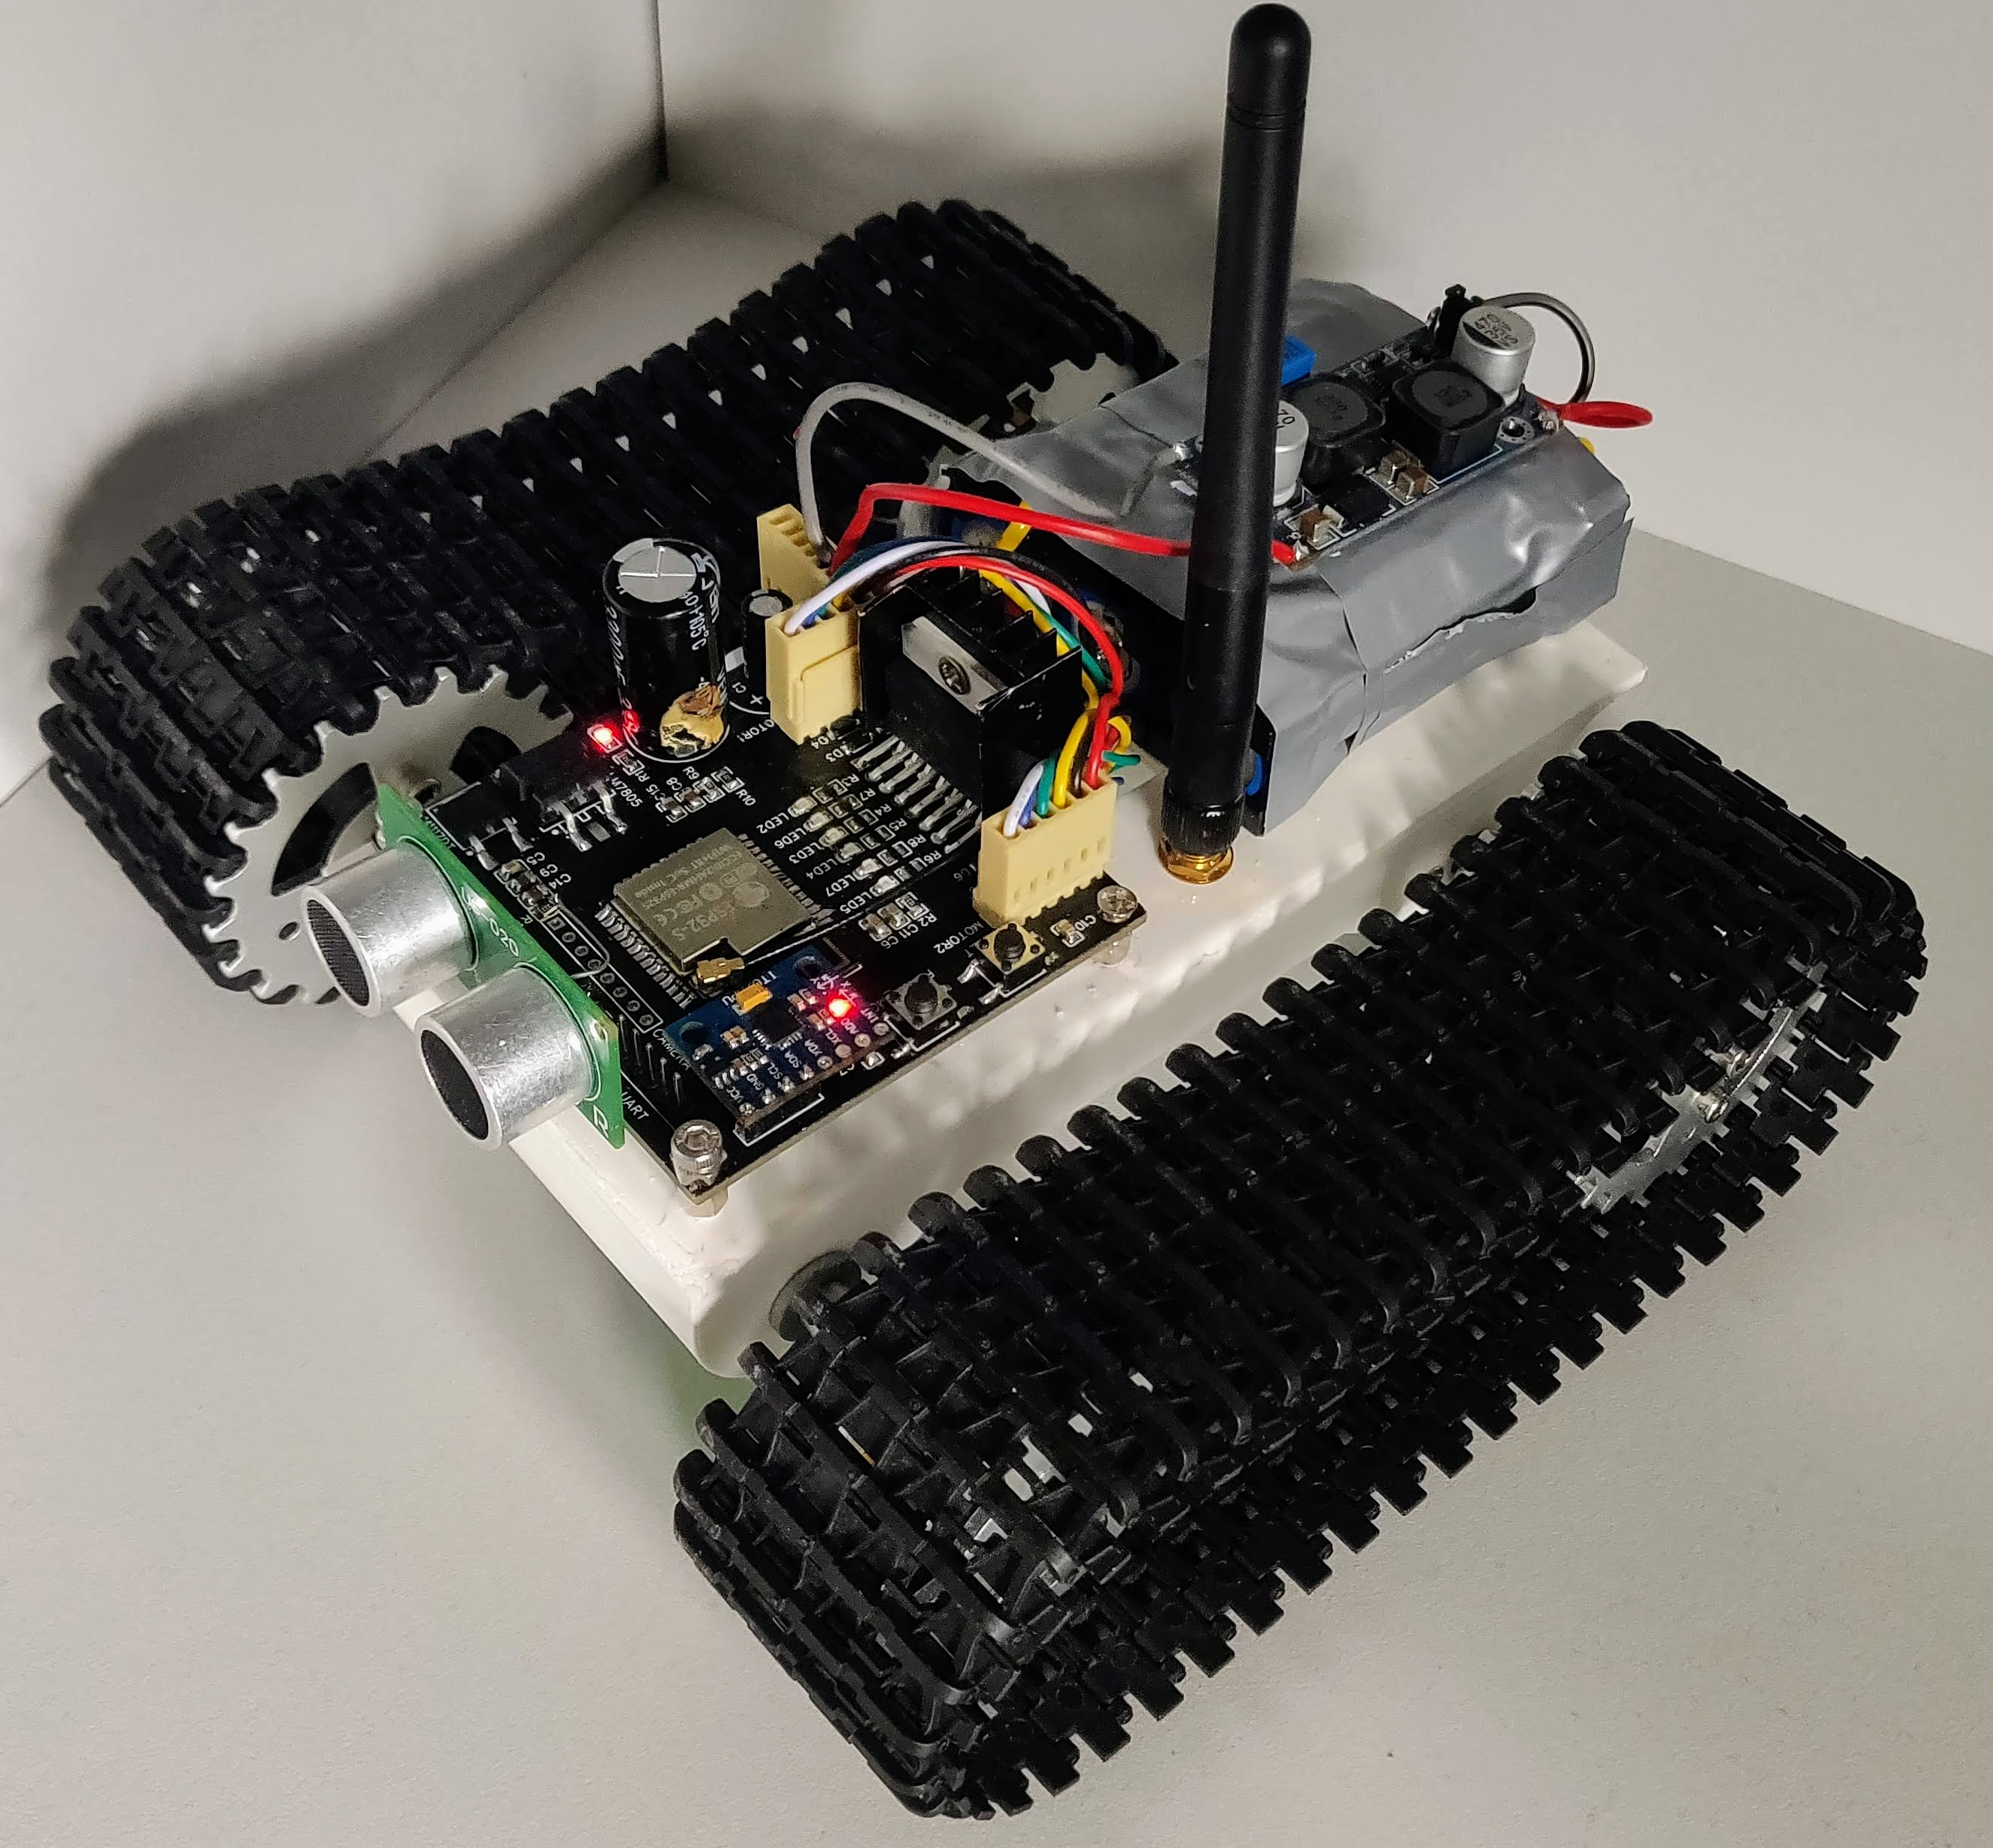
\includegraphics[width=0.7\textwidth]{figures/final/robot2.jpg}
	\caption{Ostateczna wersja robota}
	\label{fig:robot_final2}
\end{figure}

\begin{figure}[H]
	\centering
	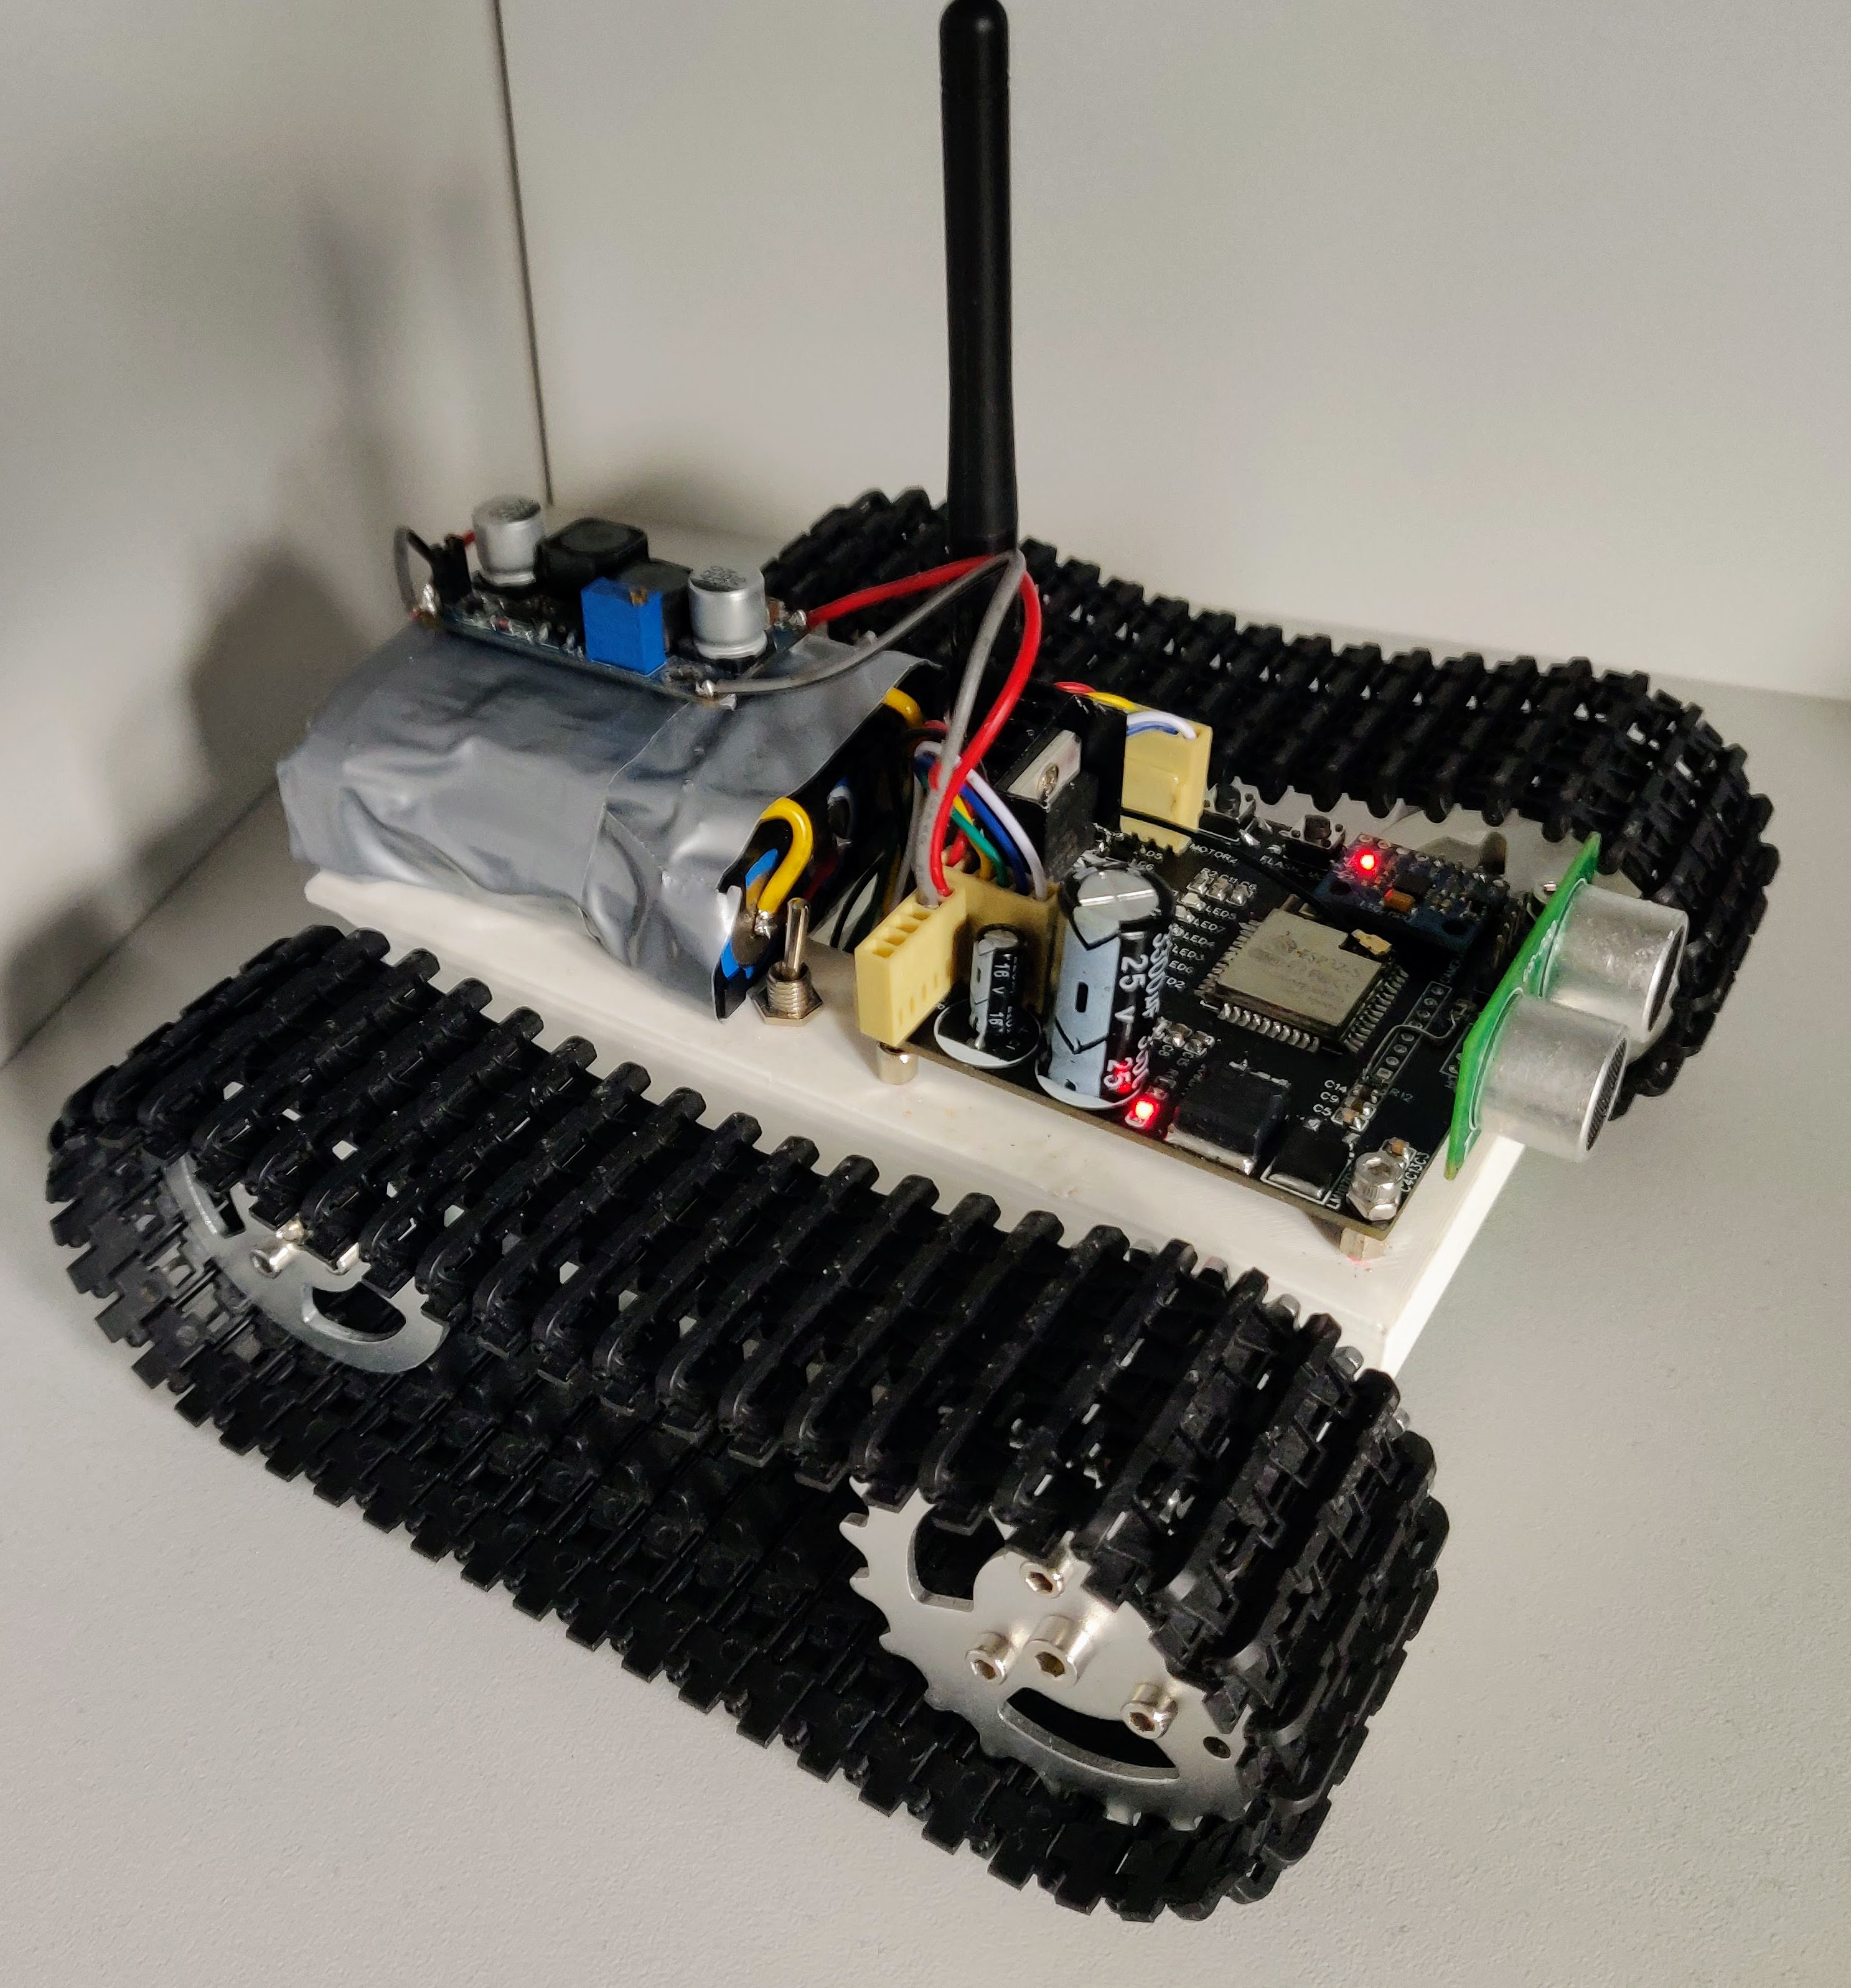
\includegraphics[width=0.65\textwidth]{figures/final/robot3.jpg}
	\caption{Ostateczna wersja robota}
	\label{fig:robot_final3}
\end{figure}

\begin{figure}[H]
	\centering
	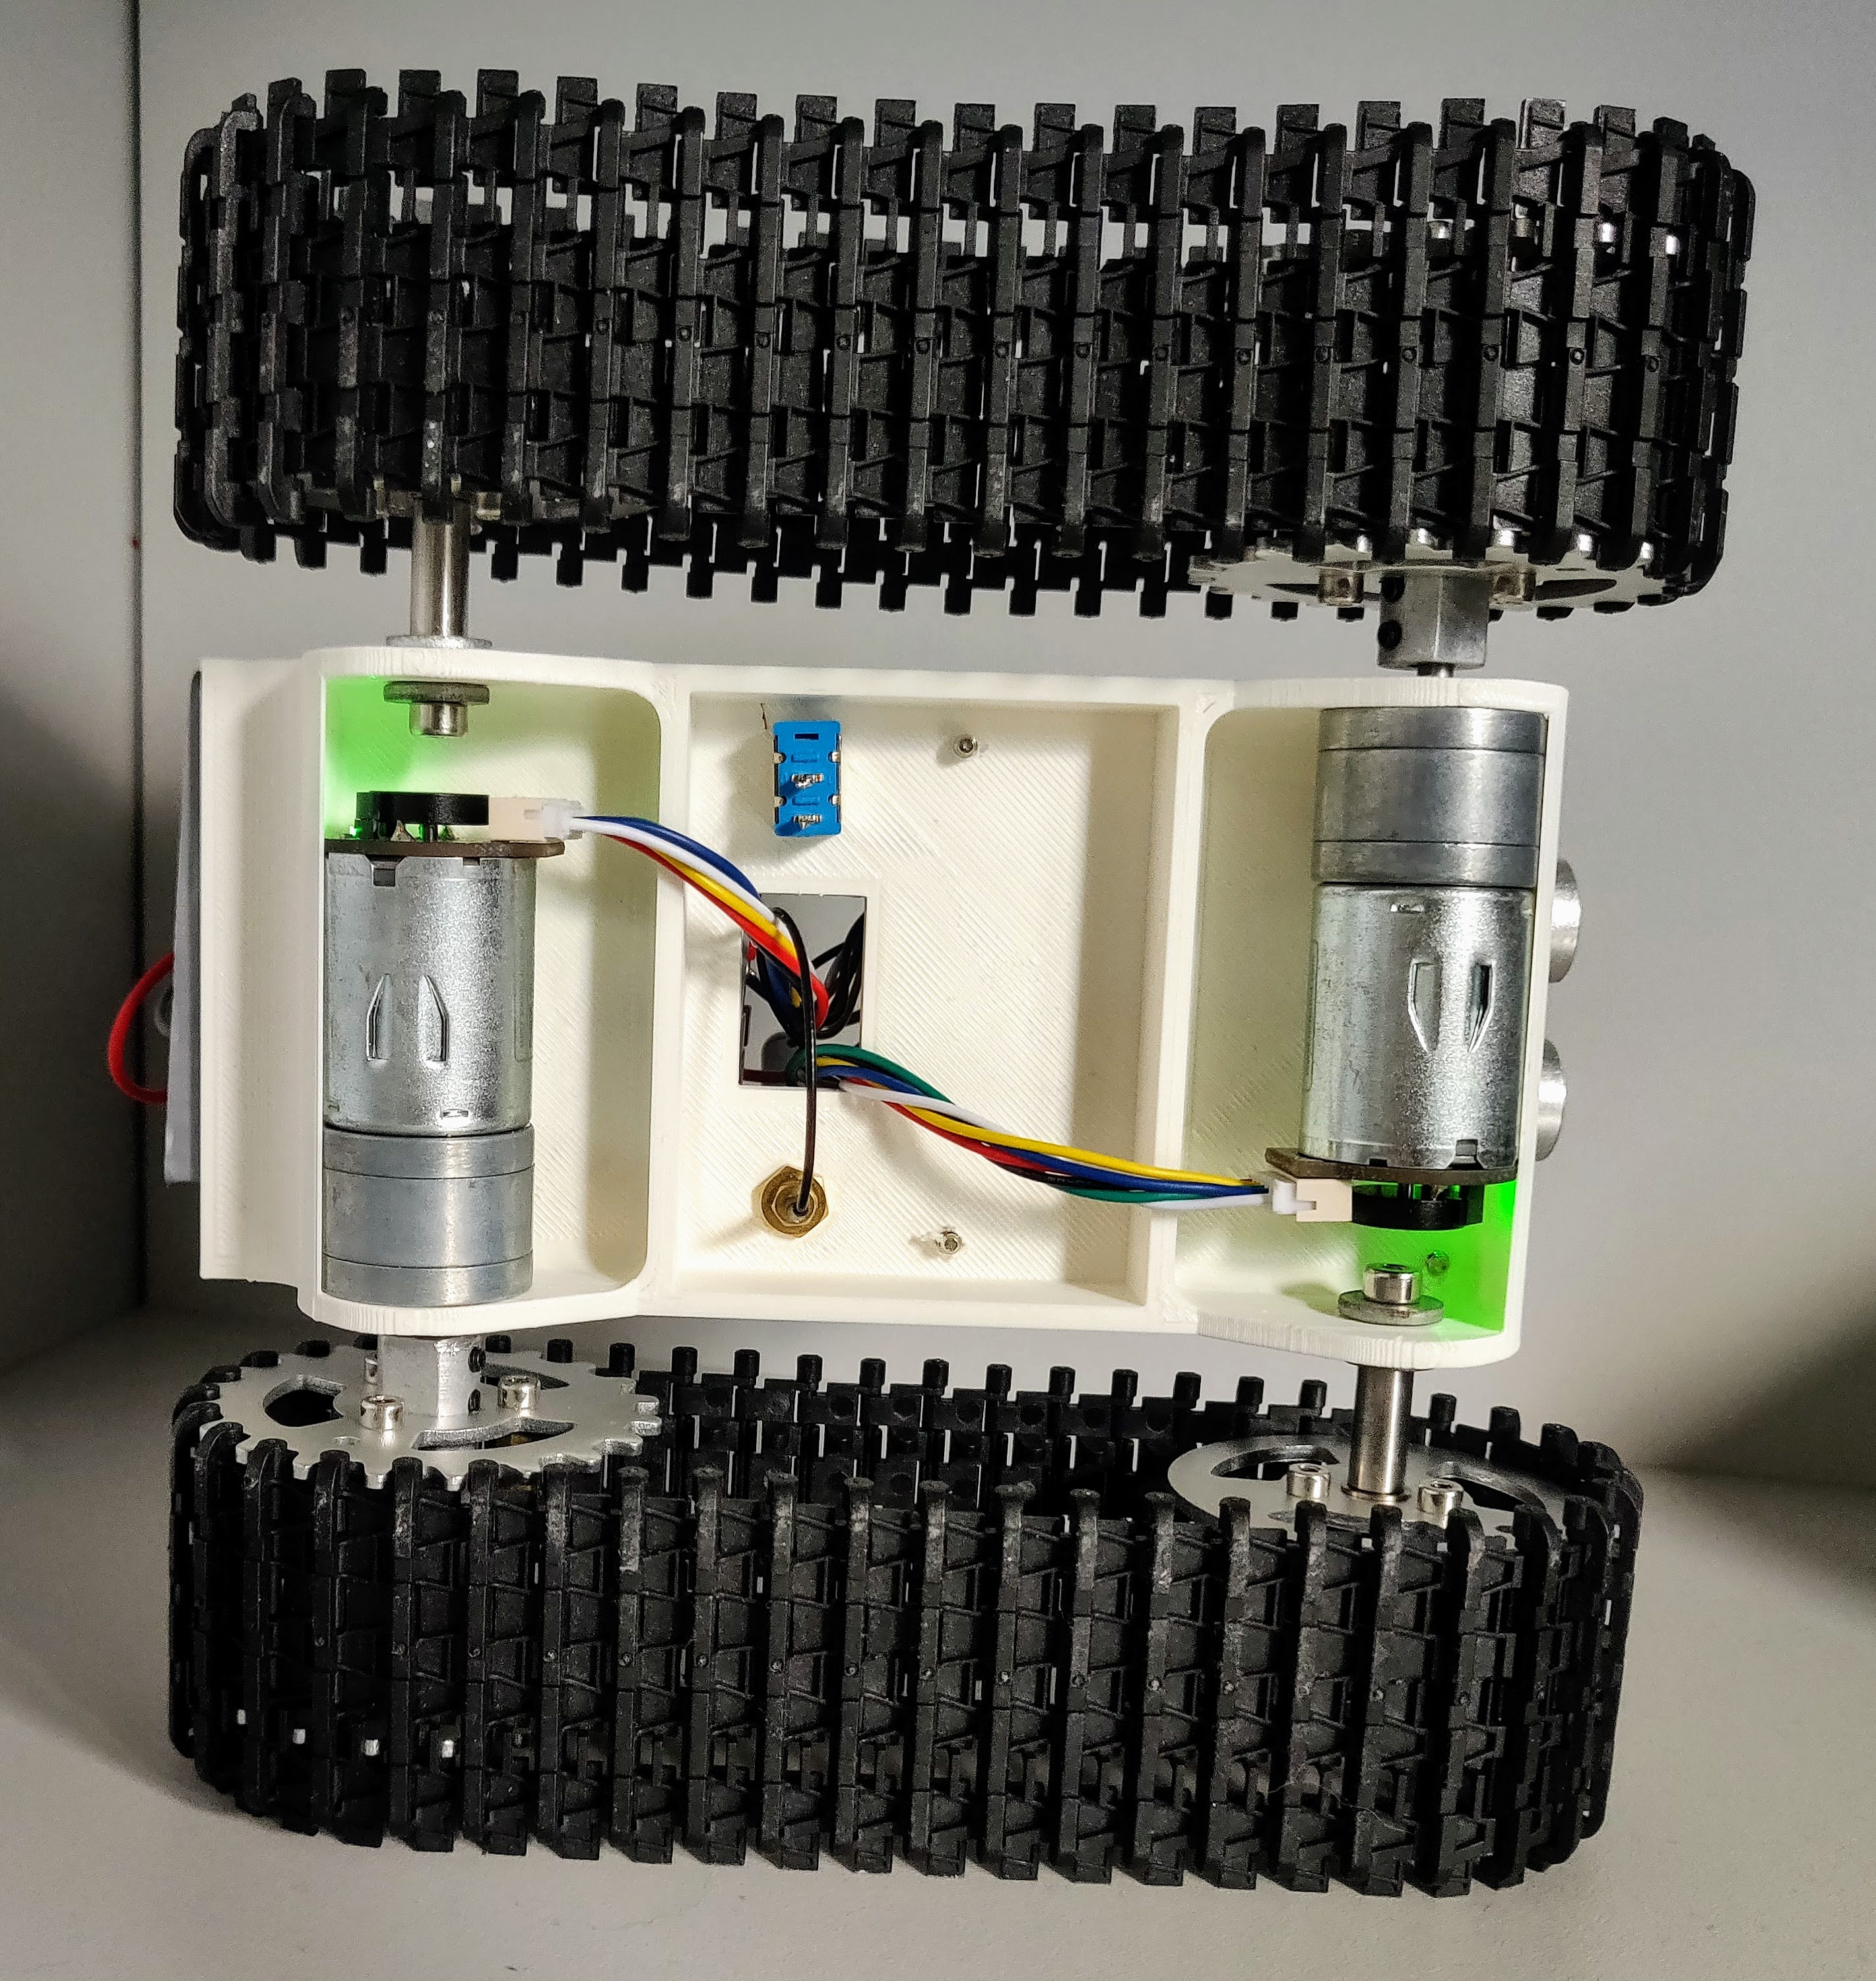
\includegraphics[width=0.7\textwidth]{figures/final/robot4.jpg}
	\caption{Ostateczna wersja robota}
	\label{fig:robot_final4}
\end{figure}

\end{document}








































